

\chapter{Intersections}\label{chap:intersections}

\section{Introduction}

The previous chapter discussed the union between two multi-structures, this chapter will discuss the intersection between two multi-structures. The important difference is that while the union required that both multi-structures have the same type, intersections can occur between structures with different types. In fact for some of the low dimensionality multi-structures such as points and paths, the intersection of two of these structure will not even be considered.

As is expected, the intersection of two structures is often the set of positions that are common to both structures, but this will not always be the case. 6 types of intersections will be considered: 
\begin{itemize}
\item point-volume intersections 
\item path-surface intersections 
\item path-volume intersections 
\item surface-surface intersections 
\item surface-volume intersections 
\item volume-volume intersections
\end{itemize}
Other intersections will not be considered, for reasons primarily related to the fact that such intersections cannot be oriented, as will be discussed later. Intersections are generally denoted with the symbol \(\cap\), but more specialized symbols will be introduced for each of the specific 6 types of intersections that are begin considered. 

\vspace{5mm}

\begin{tabular}{cc}
\parbox{0.5\textwidth}{
One property of intersections that will be used heavily is {\bf linearity}. Given a set \(A\) and two sets \(B\) and \(C\), the intersection of \(A\) with the union \(B + C\) is the sum of the intersection of \(A\) with \(B\) separately and the intersection with \(A\) with \(C\) separately. This property is referred to as ``linearity", and is also frequently referred to as the ``distributive law":

\[A \cap (B + C) = (A \cap B) + (A \cap C)\]

\[(B + C) \cap A = (B \cap A) + (C \cap A)\]

More generally if \(k\) is a real number, then the intersection of \(A\) with \(k\) copies of \(B\) is \(k\) copies of the intersection of \(A\) with \(B\):

\[A \cap (k \cdot B) = k(A \cap B)\]

\[(k \cdot A) \cap B = k(A \cap B)\]

} & \parbox{0.5\textwidth}{
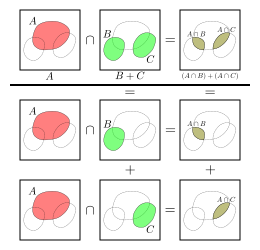
\includegraphics[width = 0.5\textwidth]{Intersections/intersection_distributive_law}
}
\end{tabular}


\section{Point-volume intersections}

Given a multi-point \(\rho\) and a multi-volume \(U\), then the intersection between \(\rho\) and \(U\) is a multi-point and is denoted by:

\[\rho \cdot U \quad\quad\text{or}\quad\quad \rho U \quad\quad\text{or}\quad\quad U \cdot \rho \quad\quad\text{or}\quad\quad U \rho\]

Given a single point \(P\), and a single volume \(\Omega\), the intersection is \(P\) if \(P\) is contained by \(\Omega\), and is nothing if \(P\) is not contained by \(\Omega\). 

If a point \(P\) with a weight of \(w_1\) is contained in a volume \(\Omega\) with a weight of \(w_2\), then for each of the \(w_2\) copies of \(\Omega\), \(w_1\) copies of \(P\) are intersecting that copy. The total intersection is \(w_1 \cdot w_2\) copies of \(P\):
\[(w_1 P) \cdot (w_2\Omega) = w_1w_2P\]      

If a point \(P\) with a weight of \(w_1\) is {\bf not} contained in a volume \(\Omega\) with a weight of \(w_2\), then for each of the \(w_2\) copies of \(\Omega\), \(w_1\) copies of \(P\) are not intersecting that copy. The total intersection is nothing:
\[(w_1 P) \cdot (w_2\Omega) = 0\]      

Given a multi-point \(\rho = w_1 P_1 + w_2 P_2 + ... + w_N P_N\) and a multi-volume \\ \(U = v_1\Omega_1 + v_2\Omega_2 + v_M\Omega_M\), then the intersection \(\rho \cdot U\) is the set of all pairwise intersections of the points and volumes:
\begin{align*}
\rho \cdot U = & \left\{\begin{array}{c}
\;\; w_1 v_1 (P_1 \cdot \Omega_1) + w_1 v_2 (P_1 \cdot \Omega_2) + \cdots + w_1 v_M (P_1 \cdot \Omega_M) \\ 
+ w_2 v_1 (P_2 \cdot \Omega_1) + w_2 v_2 (P_2 \cdot \Omega_2) + \cdots + w_2 v_M (P_2 \cdot \Omega_M) \\ 
\vdots \\
+ w_N v_1 (P_N \cdot \Omega_1) + w_N v_2 (P_N \cdot \Omega_2) + \cdots + w_N v_M (P_N \cdot \Omega_M) \\ 
\end{array}\right.
\end{align*}

In general,
\begin{itemize}
\item Given multi-points \(\rho_1\) and \(\rho_2\), and multi-volume \(U\), then:
\[(\rho_1 + \rho_2) \cdot U = \rho_1 \cdot U + \rho_2 \cdot U\] 
\item Given multi-point \(\rho\), multi-volume \(U\), and some real number \(c\), then:
\[(c\rho) \cdot U = c(\rho \cdot U)\]
\item Given multi-point \(\rho\), and multi-volumes \(U_1\) and \(U_2\), then:
\[\rho \cdot (U_1 + U_2) = \rho \cdot U_1 + \rho \cdot U_2\] 
\item Given multi-point \(\rho\), multi-volume \(U\), and some real number \(c\), then:
\[\rho \cdot (cU) = c(\rho \cdot U)\]
\end{itemize}

%Some examples of this {\bf distributive law} are listed below:
%\begin{itemize}
%\item Assume that \(P\) is contained by \(\Omega\). Given \(2\) copies of point \(P\), the intersection of the multi-point \(2P\) with the multi-volume \(\Omega\) is again 2 copies of \(P\): \((2P) \cdot \Omega = 2P\). Given an anti-copy of point \(P\), the intersection of the multi-point \(-P\) with the multi-volume \(\Omega\) is an anti-copy of \(P\): \((-P) \cdot \Omega = -P\).
%\item Assume that \(P\) is contained by \(\Omega\). Given \(2\) copies of volume \(\Omega\), the intersection of the multi-point \(P\) with the multi-volume \(2\Omega\) is again 2 copies of \(P\), since \(P\) is contained by \(2\) volumes: \(2P\). Given an anti-copy of volume \(\Omega\), the intersection of the multi-point \(P\) with the multi-volume \(-\Omega\) is an anti-copy of \(P\), since \(P\) is contained in an anti-volume: \(-P\).    
%\end{itemize}

\begin{center}
\begin{tabular}{cc}
\parbox{0.5\textwidth}{
An example of how the intersection of a multi-point and a multi-volume is the set of all pairwise intersections between the points and volumes will be given. On the right, the fact that the intersection consists of all pairs of intersections between points and volumes is illustrated with a simple example. There are two points \(P_1\) and \(P_2\), and two volumes \(\Omega_1\) and \(\Omega_2\). Points \(P_1\) and \(P_2\) are both contained in \(\Omega_1\) and \(\Omega_2\). Consider the multi-point \(\rho = P_1 + P_2\), and the multi-volume \(U = \Omega_1 + \Omega_2\). 

\(P_1\) is contained in \(\Omega_1\) so \(P_1 \cdot \Omega_1 = P_1\).  

\(P_1\) is contained in \(\Omega_2\) so \(P_1 \cdot \Omega_2 = P_1\).

\(P_2\) is contained in \(\Omega_1\) so \(P_2 \cdot \Omega_1 = P_2\).

\(P_2\) is contained in \(\Omega_2\) so \(P_2 \cdot \Omega_2 = P_2\).

The total intersection of \(\rho\) with \(U\) consists of all of the pairwise intersections:

\begin{align*}
\rho \cdot U & = P_1 + P_1 + P_2 + P_2 
= 2P_1 + 2P_2  
\end{align*}
} & \parbox{0.5\textwidth}{
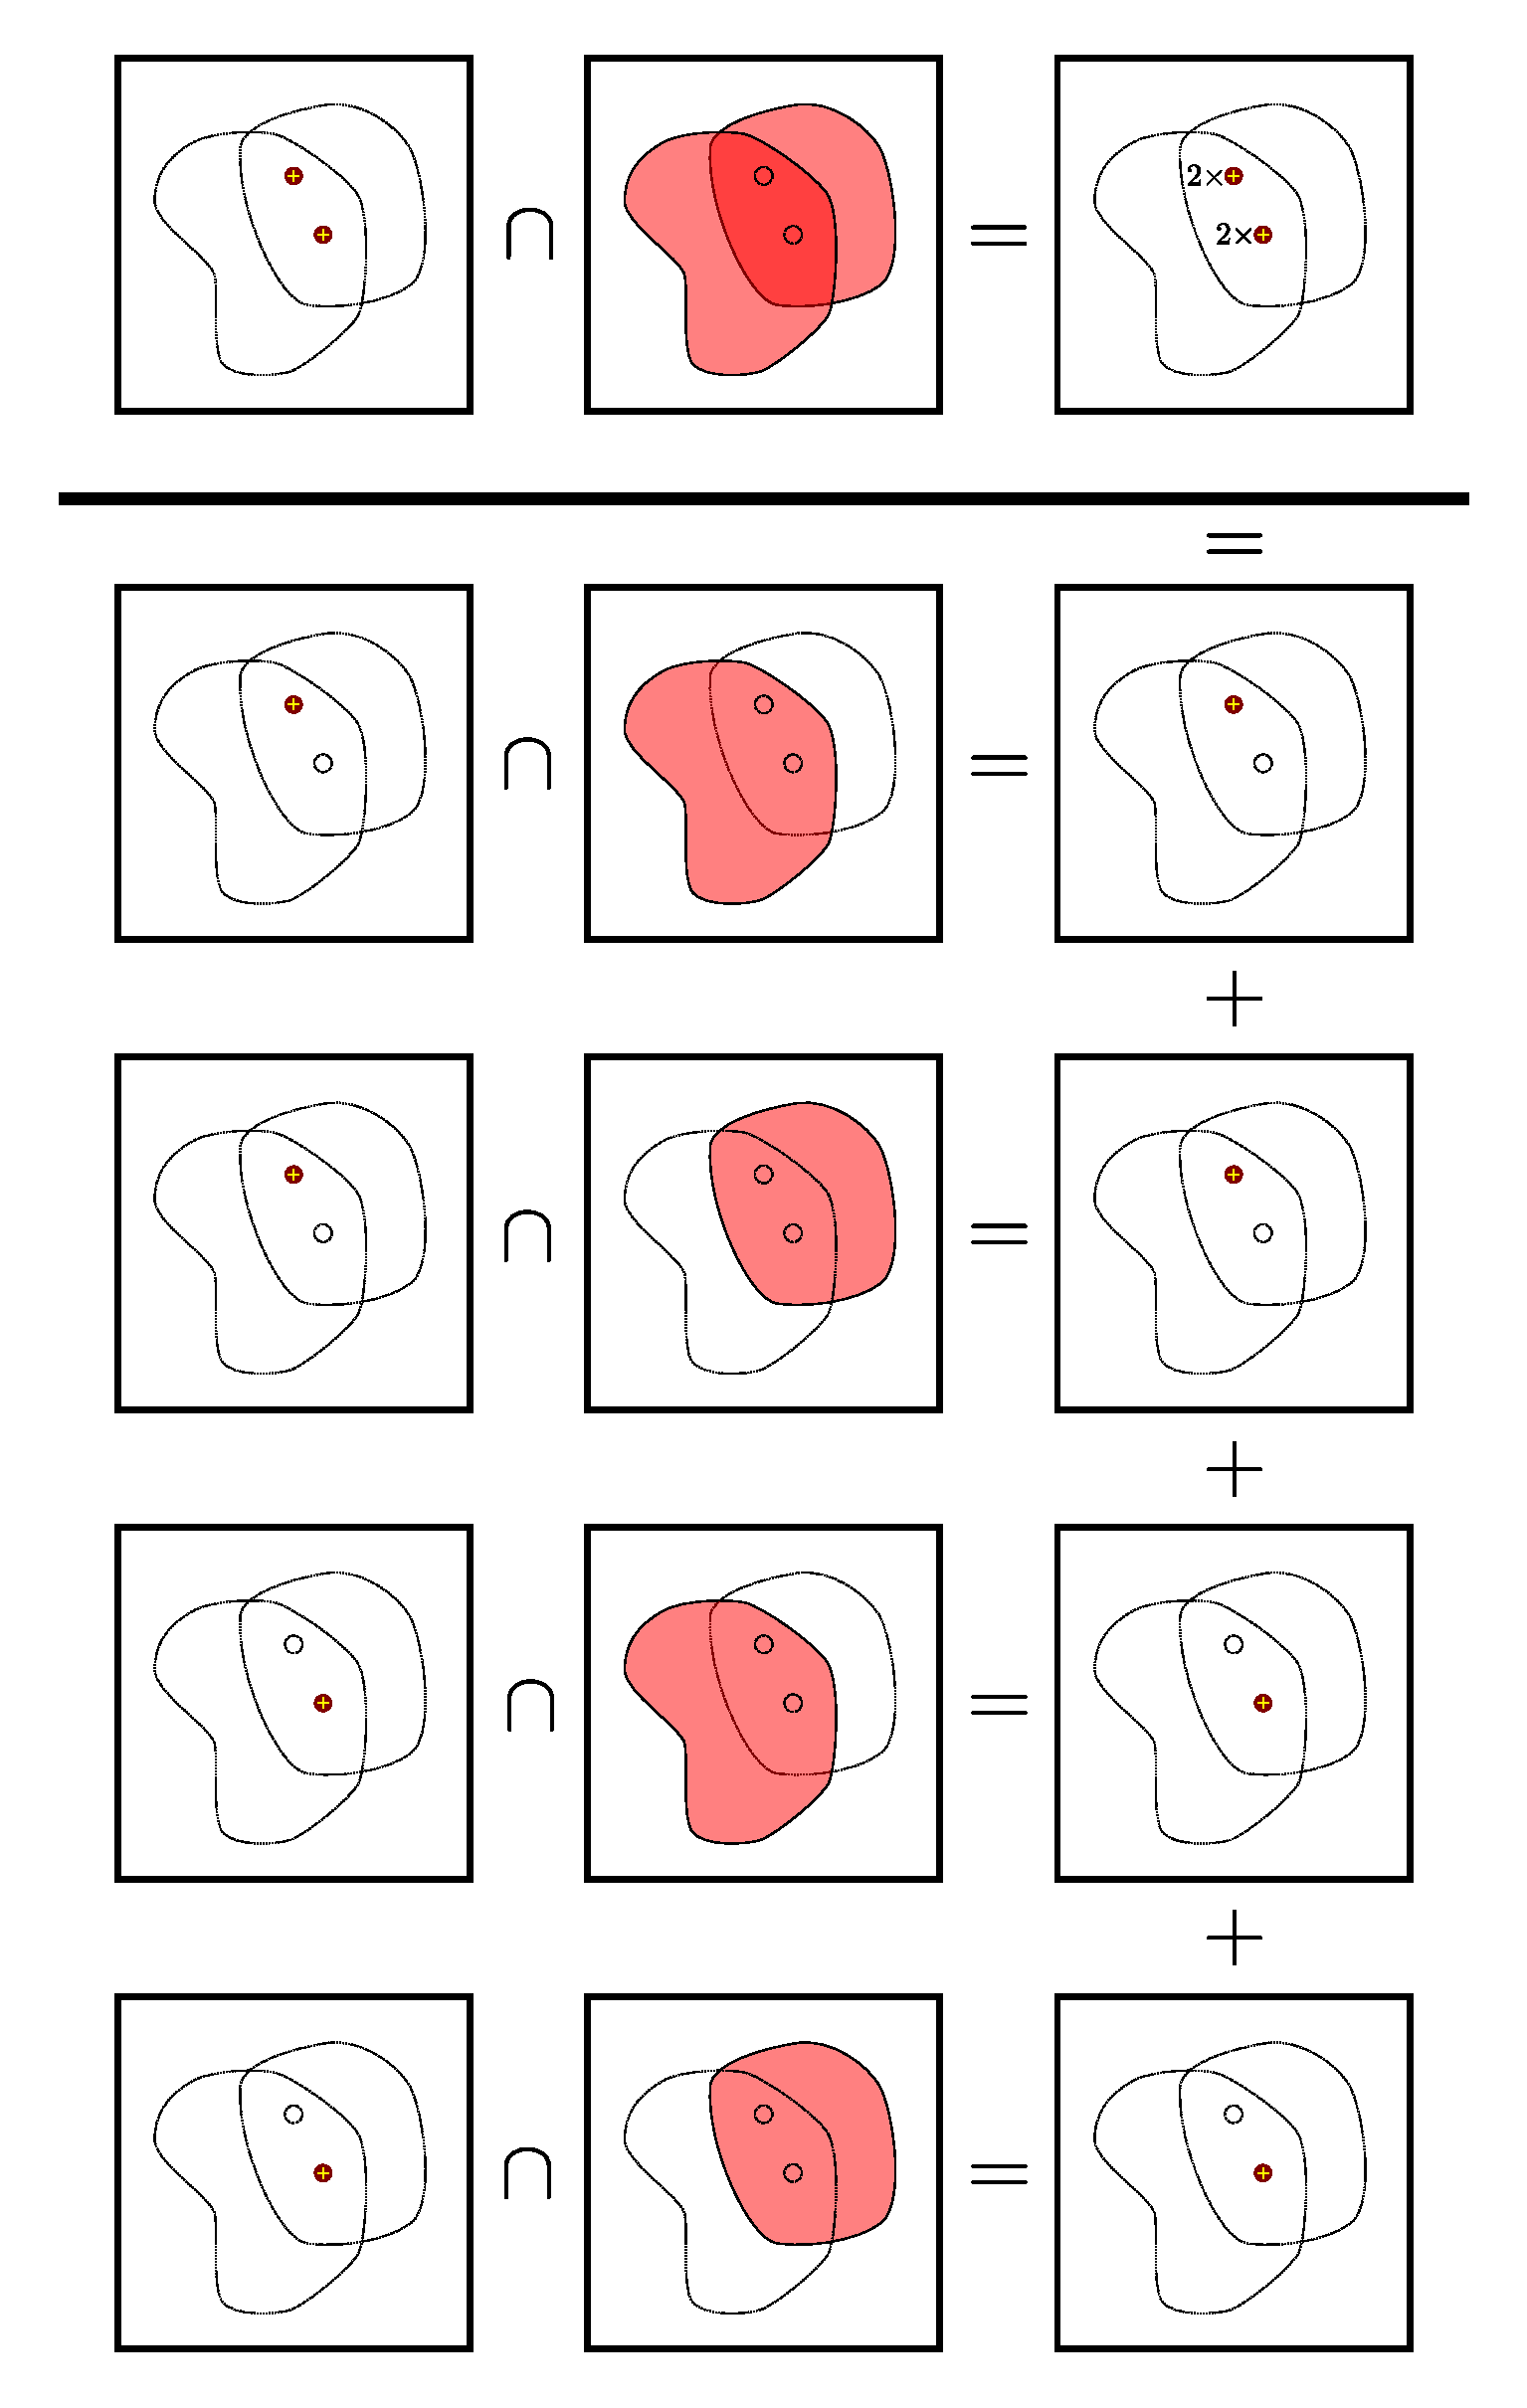
\includegraphics[width = 0.5\textwidth]{Intersections/Point-volume_intersections/point_volume_intersection_distributive_law}
}
\end{tabular}
\end{center} 

In the example below, the intersection between a multi-point and a multi-volume is illustrated. Note how the points that fall inside the negative volume have their polarities reversed. 

\begin{center}
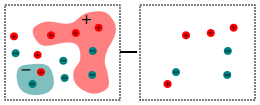
\includegraphics[scale = 0.4]{Intersections/Point-volume_intersections/point_volume_intersections_two_panel_example}
\end{center}

\begin{tabular}{cc}
\parbox{0.5\textwidth}{
If a point \(P\) with a weight of \(1\) lies on the edge of a volume with a weight of \(1\), then the intersection point \(P\) has a weight of \(0.5\).
} & \parbox{0.5\textwidth}{
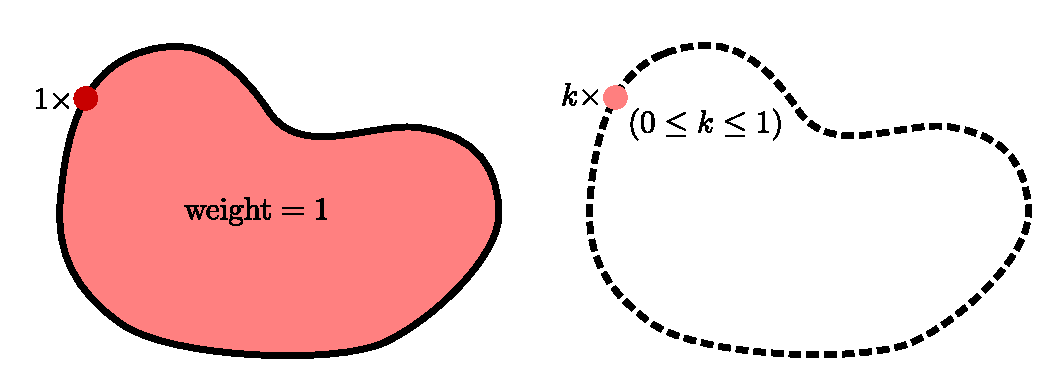
\includegraphics[width = 0.5\textwidth]{Intersections/Point-volume_intersections/point_volume_intersection_boundary_case}
}
\end{tabular}





\section{Path-surface intersections}

Given a multi-path \(\mathbf{J}\) and a multi-surface \(\mathbf{F}\), then the intersection between \(\mathbf{J}\) and \(\mathbf{F}\) is a multi-point and is denoted by:

\[\mathbf{J} \bullet \mathbf{F} \quad\quad\text{or}\quad\quad \mathbf{F} \bullet \mathbf{J}\]

An intersection occurs when a path pierces a surface. If a path with a weight of \(1\) pierces a surface with a weight of \(1\) in the preferred direction, then the intersection point has a weight of \(+1\). If a path with a weight of \(1\) pierces a surface with a weight of \(1\) in the opposite direction, then the intersection point has a weight of \(-1\). The ``preferred direction" is when the path enters the surface from the back and emerges from the front. The opposite direction is when the path enters the surface from the front and emerges from the back.

In the examples below, the intersection points have a positive weight when the path intersects the surface in the preferred direction, and the intersection points have a negative weight when the path intersects the surface in the reverse direction.

\begin{tabular}{cc}
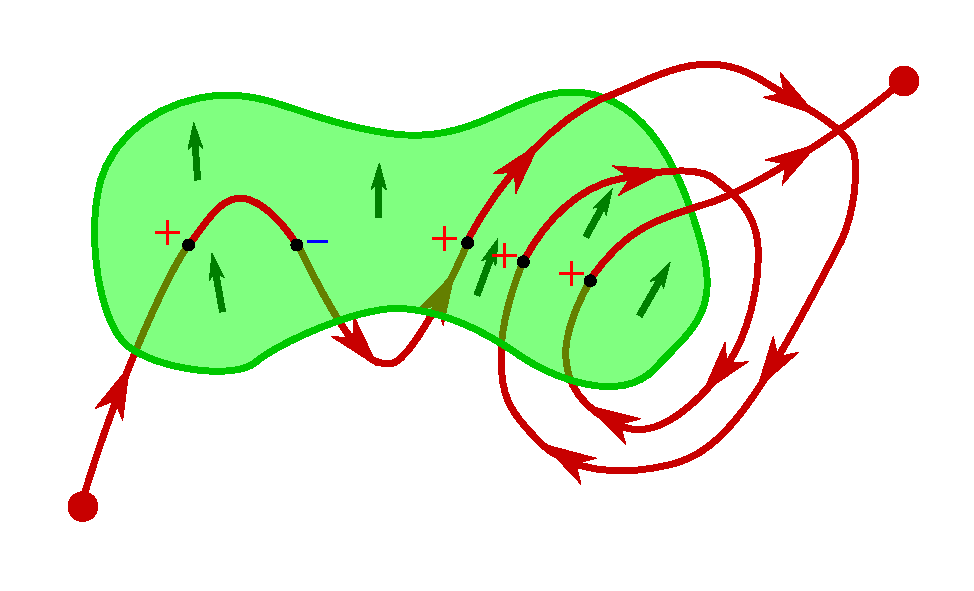
\includegraphics[width = 0.5\textwidth]{Intersections/Path-surface_intersections/path_surface_intersections}
& 
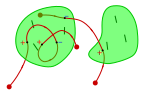
\includegraphics[width = 0.5\textwidth]{Intersections/Path-surface_intersections/path_surface_intersections_2}
\end{tabular}

If a path \(C\) with a nonnegative weight of \(w_1\) intersects a surface \(\sigma\) with a nonnegative weight of \(w_2\) in the {\bf preferred direction} at point \(P\), then for each of the \(w_2\) copies of \(\sigma\), \(w_1\) copies of \(C\) are intersecting that copy. The total intersection is \(w_1 \cdot w_2\) copies of \(P\):
\[(w_1 C) \bullet (w_2\sigma) = w_1 w_2 P\] 

Contrariwise, if a path \(C\) with a weight of \(w_1\) intersects a surface \(\sigma\) with a weight of \(w_2\) in the {\bf opposite direction} at point \(P\), then for each of the \(w_2\) copies of \(\sigma\), \(w_1\) copies of \(C\) are intersecting that copy in the opposite direction. The total intersection is \(w_1 \cdot w_2\) copies of the anti-point \(-P\):
\[(w_1 C) \bullet (w_2 \sigma) = -w_1 w_2 P\]  

Given a multi-path \(\mathbf{J} = w_1C_1 + w_2C_2 + ... + w_NC_N\) and a multi-surface \\ \(\mathbf{F} = v_1\sigma_1 + v_2\sigma_2 + ... + v_M\sigma_M\), then the intersection \(\mathbf{J} \bullet \mathbf{F}\) is the set of all pairwise intersections of the paths and surfaces:
\begin{align*}
\mathbf{J} \bullet \mathbf{F} = & \left\{\begin{array}{c}
\;\; w_1 v_1 (C_1 \bullet \sigma_1) + w_1 v_2 (C_1 \bullet \sigma_2) + \cdots + w_1 v_M (C_1 \bullet \sigma_M) \\ 
+ w_2 v_1 (C_2 \bullet \sigma_1) + w_2 v_2 (C_2 \bullet \sigma_2) + \cdots + w_2 v_M (C_2 \bullet \sigma_M) \\ 
\vdots \\
+ w_N v_1 (C_N \bullet \sigma_1) + w_N v_2 (C_N \bullet \sigma_2) + \cdots + w_N v_M (C_N \bullet \sigma_M) \\ 
\end{array}\right.
\end{align*}

In general,
\begin{itemize}
\item Given multi-paths \(\mathbf{J}_1\) and \(\mathbf{J}_2\), and multi-surface \(\mathbf{F}\), then:
\[(\mathbf{J}_1 + \mathbf{J}_2) \bullet \mathbf{F} = \mathbf{J}_1 \bullet \mathbf{F} + \mathbf{J}_2 \bullet \mathbf{F}\] 
\item Given multi-path \(\mathbf{J}\), multi-surface \(\mathbf{F}\), and some real number \(c\), then:
\[(c\mathbf{J}) \bullet \mathbf{F} = c(\mathbf{J} \bullet \mathbf{F})\]
\item Given multi-path \(\mathbf{J}\), and multi-surfaces \(\mathbf{F}_1\) and \(\mathbf{F}_2\), then:
\[\mathbf{J} \bullet (\mathbf{F}_1 + \mathbf{F}_2) = \mathbf{J} \bullet \mathbf{F}_1 + \mathbf{J} \bullet \mathbf{F}_2\] 
\item Given multi-path \(\mathbf{J}\), multi-surface \(\mathbf{F}\), and some real number \(c\), then:
\[\mathbf{J} \bullet (c\mathbf{F}) = c(\mathbf{J} \bullet \mathbf{F})\]
\end{itemize}

\begin{center}
\begin{tabular}{cc}
\parbox{0.5\textwidth}{
An example of how the intersection of a multi-path and a multi-surface is the set of all pairwise intersections between the paths and surfaces will be given. On the right, the fact that the intersection consists of all pairs of intersections between paths and surfaces is illustrated with a simple example. There are two oriented paths \(C_1\) and \(C_2\), and two oriented surfaces \(\sigma_1\) and \(\sigma_2\). Paths \(C_1\) and \(C_2\) both pass through \(\sigma_1\) and \(\sigma_2\) in the preferred direction. Consider the multi-path \(\mathbf{J} = C_1 + C_2\), and the multi-surface \(\mathbf{F} = \sigma_1 + \sigma_2\). 

The intersection of \(C_1\) with \(\sigma_1\) is a point \(P_{1,1}\) so \\ \(C_1 \bullet \sigma_1 = P_{1,1}\)  

The intersection of \(C_1\) with \(\sigma_2\) is a point \(P_{1,2}\) so \\ \(C_1 \bullet \sigma_2 = P_{1,2}\)  

The intersection of \(C_2\) with \(\sigma_1\) is a point \(P_{2,1}\) so \\ \(C_2 \bullet \sigma_1 = P_{2,1}\)  

The intersection of \(C_2\) with \(\sigma_2\) is a point \(P_{2,2}\) so \\ \(C_2 \bullet \sigma_2 = P_{2,2}\)  

The total intersection of \(\mathbf{J}\) with \(\mathbf{F}\) consists of all of the pairwise intersections:

\begin{align*}
\mathbf{J} \bullet \mathbf{F} & = P_{1,1} + P_{1,2} + P_{2,1} + P_{2,2} 
\end{align*}
} & \parbox{0.4\textwidth}{
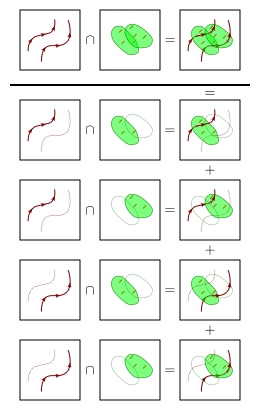
\includegraphics[width = 0.4\textwidth]{Intersections/Path-surface_intersections/path_surface_intersection_distributive_law}
}
\end{tabular}
\end{center}

If a path \(C\) fails to fully pass through a surface \(\sigma\), then the weight of the intersection point is halved. {\bf Paths that are embedded inside of surfaces do contribute any intersection points unless they enter or leave the surface.} It may be argued that all points along an embedded path should be counted as intersection points, but the counter argument is to ask what polarity these points should have.

If path \(C\) enters the back of \(\sigma\) and then continues inside of \(\sigma\), then the point where \(C\) first touches \(\sigma\) has a weight of \(+0.5\). If path \(C\) enters the front of \(\sigma\) and then continues inside of \(\sigma\), then the point where \(C\) first touches \(\sigma\) has a weight of \(-0.5\). 

If \(C\) is inside of \(\sigma\) and then exits the front of \(\sigma\), then the exit point has a weight of \(+0.5\). If \(C\) is inside of \(\sigma\) and then exits the back of \(\sigma\), then the exit point has a weight of \(-0.5\). 

\begin{center}
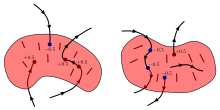
\includegraphics[width = 0.75\textwidth]{Intersections/Path-surface_intersections/path_surface_intersection_boundary_case}
\end{center}

Moreover, if the path \(C\) clips the boundary of \(\sigma\), then the weight of the intersection point is also halved.





\section{Path-volume intersections}

Given a multi-path \(\mathbf{J}\) and a multi-volume \(U\), then the intersection between \(\mathbf{J}\) and \(U\) is a multi-path and is denoted by:

\[\mathbf{J} \cdot U \quad\quad\text{or}\quad\quad \mathbf{J} U \quad\quad\text{or}\quad\quad U \cdot \mathbf{J} \quad\quad\text{or}\quad\quad U \mathbf{J}\]

Given an oriented path \(C\), and a volume \(\Omega\), then the intersection is the sections of \(C\) that are contained in \(\Omega\). If the weight of \(\Omega\) is negative, then the orientation of the intersection is reversed. % The intersection is the sections of \(\mathbf{J}\) that are embedded in \(\mathbf{U}\). If the volume 

In the examples below, only sections of the path that are contained inside a volume are part of the intersection.

\begin{center}
\begin{tabular}{cc}
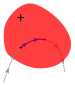
\includegraphics[width = 0.3\textwidth]{Intersections/Path-volume_intersections/path_volume_intersections_example}
& 
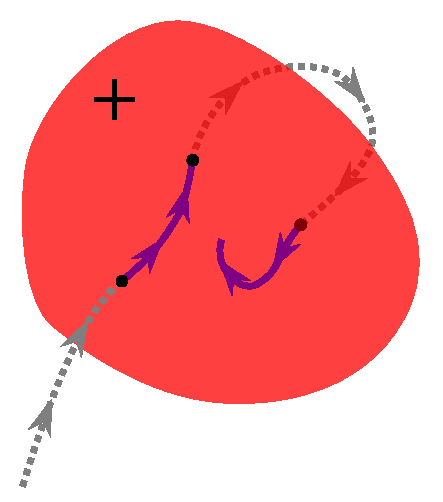
\includegraphics[width = 0.3\textwidth]{Intersections/Path-volume_intersections/path_volume_intersections_example_2}
\end{tabular}
\end{center}

If a path \(C\) with a nonnegative weight of \(w_1\) intersects a volume \(\Omega\) with a weight of \(w_2\), and \(C'\) is the sections of \(C\) that are contained in \(\Omega\), then for each of the \(w_2\) copies of \(\Omega\), \(w_1\) copies of \(C\) are intersecting that copy. The total intersection is \(w_1 \cdot w_2\) copies of \(C'\):
\[(w_1 C) \cdot (w_2 \Omega) = w_1 w_2 C'\] 
If the volume weight \(w_2\) is negative, then both the orientation of \(C'\) and the sign of the weight \(w_1 w_2\) is flipped. 

Given a multi-path \(\mathbf{J} = w_1 C_1 + w_2 C_2 + ... + w_N C_N\) and a multi-volume \\ \(U = v_1 \Omega_1 + v_2\Omega_2 + ... + v_M\Omega_M\), then the intersection \(\mathbf{J} \cdot U\) is the set of all pairwise intersections of the paths and volumes:
\begin{align*}
\mathbf{J} \cdot U = & \left\{\begin{array}{c}
\;\; w_1 v_1 (C_1 \cdot \Omega_1) + w_1 v_2 (C_1 \cdot \Omega_2) + \cdots + w_1 v_M (C_1 \cdot \Omega_M) \\ 
+ w_2 v_1 (C_2 \cdot \Omega_1) + w_2 v_2 (C_2 \cdot \Omega_2) + \cdots + w_2 v_M (C_2 \cdot \Omega_M) \\ 
\vdots \\
+ w_N v_1 (C_N \cdot \Omega_1) + w_N v_2 (C_N \cdot \Omega_2) + \cdots + w_N v_M (C_N \cdot \Omega_M) \\ 
\end{array}\right.
\end{align*}

In general,
\begin{itemize}
\item Given multi-paths \(\mathbf{J}_1\) and \(\mathbf{J}_2\), and multi-volume \(U\), then:
\[(\mathbf{J}_1 + \mathbf{J}_2) \cdot U = \mathbf{J}_1 \cdot U + \mathbf{J}_2 \cdot U\] 
\item Given multi-path \(\mathbf{J}\), multi-volume \(U\), and some real number \(c\), then:
\[(c\mathbf{J}) \cdot U = c(\mathbf{J} \cdot U)\]
\item Given multi-path \(\mathbf{J}\), and multi-volumes \(U_1\) and \(U_2\), then:
\[\mathbf{J} \cdot (U_1 + U_2) = \mathbf{J} \cdot U_1 + \mathbf{J} \cdot U_2\] 
\item Given multi-path \(\mathbf{J}\), multi-volume \(U\), and some real number \(c\), then:
\[\mathbf{J} \cdot (cU) = c(\mathbf{J} \cdot U)\]
\end{itemize}

In the example below, the multi-volume \(U\) consists of three volumes. Two of the volumes have a weight of \(+1\) and are overlapping, and the remaining separate volume has a weight of \(-1\). The multi-path \(\mathbf{J}\) consists of a single path that winds through each of the volumes. Outside of all of the volumes, the path is not part of the intersection. Where the path is passing through a single volume with a weight of \(+1\), the intersection path from \(\mathbf{J} \cdot U\) has a weight of \(+1\). Where the path is passing through the overlap between the volumes with a weight of \(+1\), then each volume contributes a copy of the intersection to \(\mathbf{J} \cdot U\) so the weight of the path in \(\mathbf{J} \cdot U\) is \(+2\). Where the path is passing through the volume with a weight of \(-1\), the orientation of the intersection is reversed.  

\begin{center}
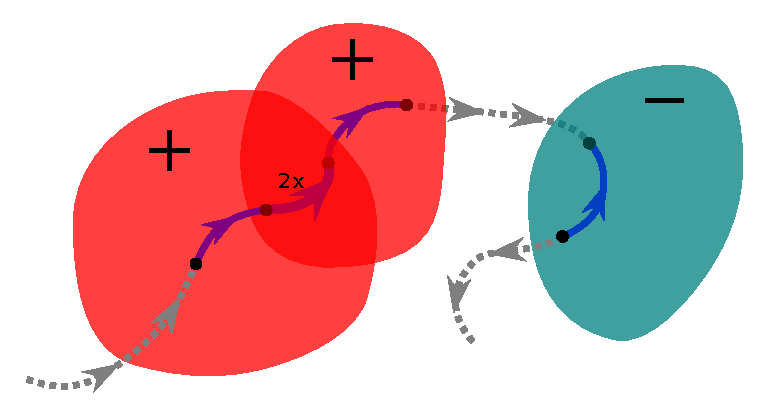
\includegraphics[width = 0.75\textwidth]{Intersections/Path-volume_intersections/path_volume_intersections_example_3}
\end{center}


\begin{tabular}{cc}
\parbox{0.5\textwidth}{
If a path \(C\) is on the surface of volume \(\Omega\), then the intersection is \(C\) with a weight of \(+0.5\) as depicted on the right.
} & \parbox{0.5\textwidth}{
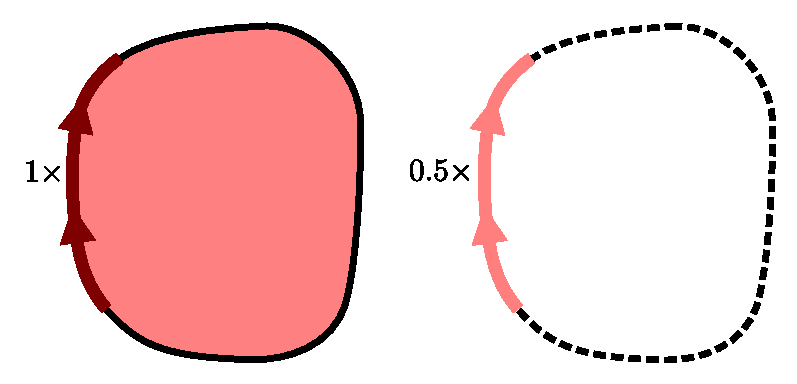
\includegraphics[width = 0.5\textwidth]{Intersections/Path-volume_intersections/path_volume_intersection_boundary_case}
}
\end{tabular}






\section{Surface-surface intersections}

Given two multi-surfaces \(\mathbf{F}_1\) and \(\mathbf{F}_2\), then the intersection between \(\mathbf{F}_1\) and \(\mathbf{F}_2\) is a multi-path and is denoted by:

\[\mathbf{F}_1 \times \mathbf{F}_2\]

An intersection occurs when a surface slices into another surface along a curve. The orientation of the intersection curve is now to be determined. 

\begin{tabular}{cc}
\parbox{0.5\textwidth}{
Given two oriented surfaces \(\sigma_1\) and \(\sigma_2\), the orientation of the intersection \(C\) can be determined as follows. Position your view point in the space that contains the front of \(\sigma_1\) and \(\sigma_2\). When the \(\sigma_1\) is on your left, and \(\sigma_2\) is on your right, then the intersection is oriented towards you as depicted on the right. This is commonly referred to as the ``righthand rule".
} & \parbox{0.5\textwidth}{
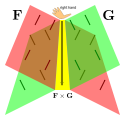
\includegraphics[width = 0.5\textwidth]{Intersections/Surface-surface_intersections/right_hand_rule}
}
\end{tabular}

Some examples are shown below:

\begin{center}
\begin{tabular}{cc}
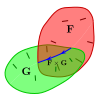
\includegraphics[width = 0.4\textwidth]{Intersections/Surface-surface_intersections/surface_surface_intersections_example}
& 
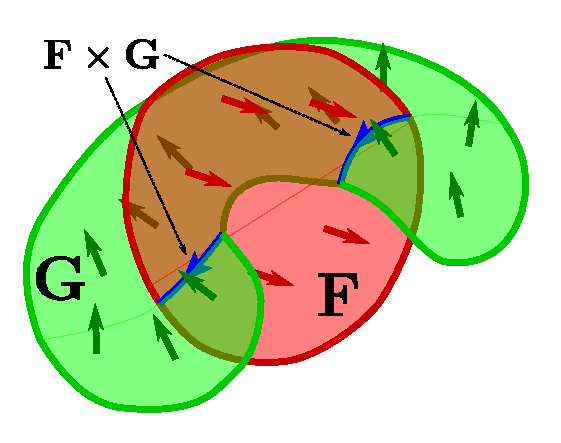
\includegraphics[width = 0.4\textwidth]{Intersections/Surface-surface_intersections/surface_surface_intersections_example_2}
\end{tabular}
\end{center}

Unlike other intersections, the ``order" of the two surfaces impacts the orientation of the intersection path. If the order of the surfaces is reversed, then the orientation of the intersection path is also reversed:

\[\sigma_2 \cap \sigma_1 = -(\sigma_1 \cap \sigma_2)\]

so:

\begin{thm}
Given any multi-surfaces \(\mathbf{F}_1\) and \(\mathbf{F}_2\), then:
\[\mathbf{F}_2 \times \mathbf{F}_1 = -(\mathbf{F}_1 \times \mathbf{F}_2)\]
\end{thm}

If a surface \(\sigma_1\) with a nonnegative weight of \(w_1\) intersects a surface \(\sigma_2\) with a nonnegative weight of \(w_2\) along the path \(C\) according to the righthand rule, then for each of the \(w_2\) copies of \(\sigma_2\), \(w_1\) copies of \(\sigma_1\) are intersecting that copy. The total intersection is \(w_1 \cdot w_2\) copies of \(C\):
\[(w_1 \sigma_1) \times (w_2 \sigma_2) = w_1 w_2 C\] 

Given multi-surfaces \(\mathbf{F}_1 = w_1\sigma_1 + w_2\sigma_2 + ... + w_N\sigma_N\) and \\ \(\mathbf{F}_2 = v_1\tau_1 + v_2\tau_2 + ... + v_M\tau_M\), then the intersection \(\mathbf{F}_1 \times \mathbf{F}_2\) is the set of all pairwise intersections of the surfaces:
\begin{align*}
\mathbf{F}_1 \times \mathbf{F}_2 = & \left\{\begin{array}{c}
\;\; w_1 v_1 (\sigma_1 \times \tau_1) + w_1 v_2 (\sigma_1 \times \tau_2) + \cdots + w_1 v_M (\sigma_1 \times \tau_M) \\ 
+ w_2 v_1 (\sigma_2 \times \tau_1) + w_2 v_2 (\sigma_2 \times \tau_2) + \cdots + w_2 v_M (\sigma_2 \times \tau_M) \\ 
\vdots \\
+ w_N v_1 (\sigma_N \times \tau_1) + w_N v_2 (\sigma_N \times \tau_2) + \cdots + w_N v_M (\sigma_N \times \tau_M) \\ 
\end{array}\right.
\end{align*}

In general,
\begin{itemize}
\item Given multi-surfaces \(\mathbf{F}_1\), \(\mathbf{F}_2\), and \(\mathbf{G}\), then:
\[(\mathbf{F}_1 + \mathbf{F}_2) \times \mathbf{G} = \mathbf{F}_1 \times \mathbf{G} + \mathbf{F}_2 \times \mathbf{G}\] 
\item Given multi-surfaces \(\mathbf{F}\) and \(\mathbf{G}\), and some real number \(c\), then:
\[(c\mathbf{F}) \times \mathbf{G} = c(\mathbf{F} \times \mathbf{G})\]
\item Given multi-surfaces \(\mathbf{F}\), \(\mathbf{G}_1\), and \(\mathbf{G}_2\), then:
\[\mathbf{F} \times (\mathbf{G}_1 + \mathbf{G}_2) = \mathbf{F} \times \mathbf{G}_1 + \mathbf{F} \times \mathbf{G}_2\] 
\item Given multi-surfaces \(\mathbf{F}\) and \(\mathbf{G}\), and some real number \(c\), then:
\[\mathbf{F} \times (c\mathbf{G}) = c(\mathbf{F} \times \mathbf{G})\]
\end{itemize}

\begin{center}
\begin{tabular}{cc}
\parbox{0.5\textwidth}{
An example of how the intersection of two multi-surfaces is the set of all pairwise intersections between the surfaces will be given. On the right, the fact that the intersection consists of all pairs of intersections between surfaces from the two multi-surfaces is illustrated with a simple example. There are four oriented surfaces \(\sigma_1\), \(\sigma_2\) (in the \(1^\text{st}\) column, and \(\tau_1\), \(\tau_2\) (in the \(2^\text{nd}\) column). Surfaces \(\sigma_1\) and \(\sigma_2\) both slice into \(\tau_1\) and \(\tau_2\). Consider the multi-surface \(\mathbf{F}_1 = \sigma_1 + \sigma_2\), and the multi-surface \(\mathbf{F}_2 = \tau_1 + \tau_2\). 

The intersection of \(\sigma_1\) with \(\tau_1\) is an oriented curve \(C_{1,1}\) so \(\sigma_1 \times \tau_1 = C_{1,1}\).  

The intersection of \(\sigma_1\) with \(\tau_2\) is an oriented curve \(C_{1,2}\) so \(\sigma_1 \times \tau_2 = C_{1,2}\).  

The intersection of \(\sigma_2\) with \(\tau_1\) is an oriented curve \(C_{2,1}\) so \(\sigma_2 \times \tau_1 = C_{2,1}\).   

The intersection of \(\sigma_2\) with \(\tau_2\) is an oriented curve \(C_{2,2}\) so \(\sigma_2 \times \tau_2 = C_{2,2}\).     

The total intersection of \(\mathbf{F}_1\) with \(\mathbf{F}_2\) consists of all of the pairwise intersections:

\begin{align*}
\mathbf{F}_1 \times \mathbf{F}_2 & = C_{1,1} + C_{1,2} + C_{2,1} + C_{2,2} 
\end{align*}
} & \parbox{0.4\textwidth}{
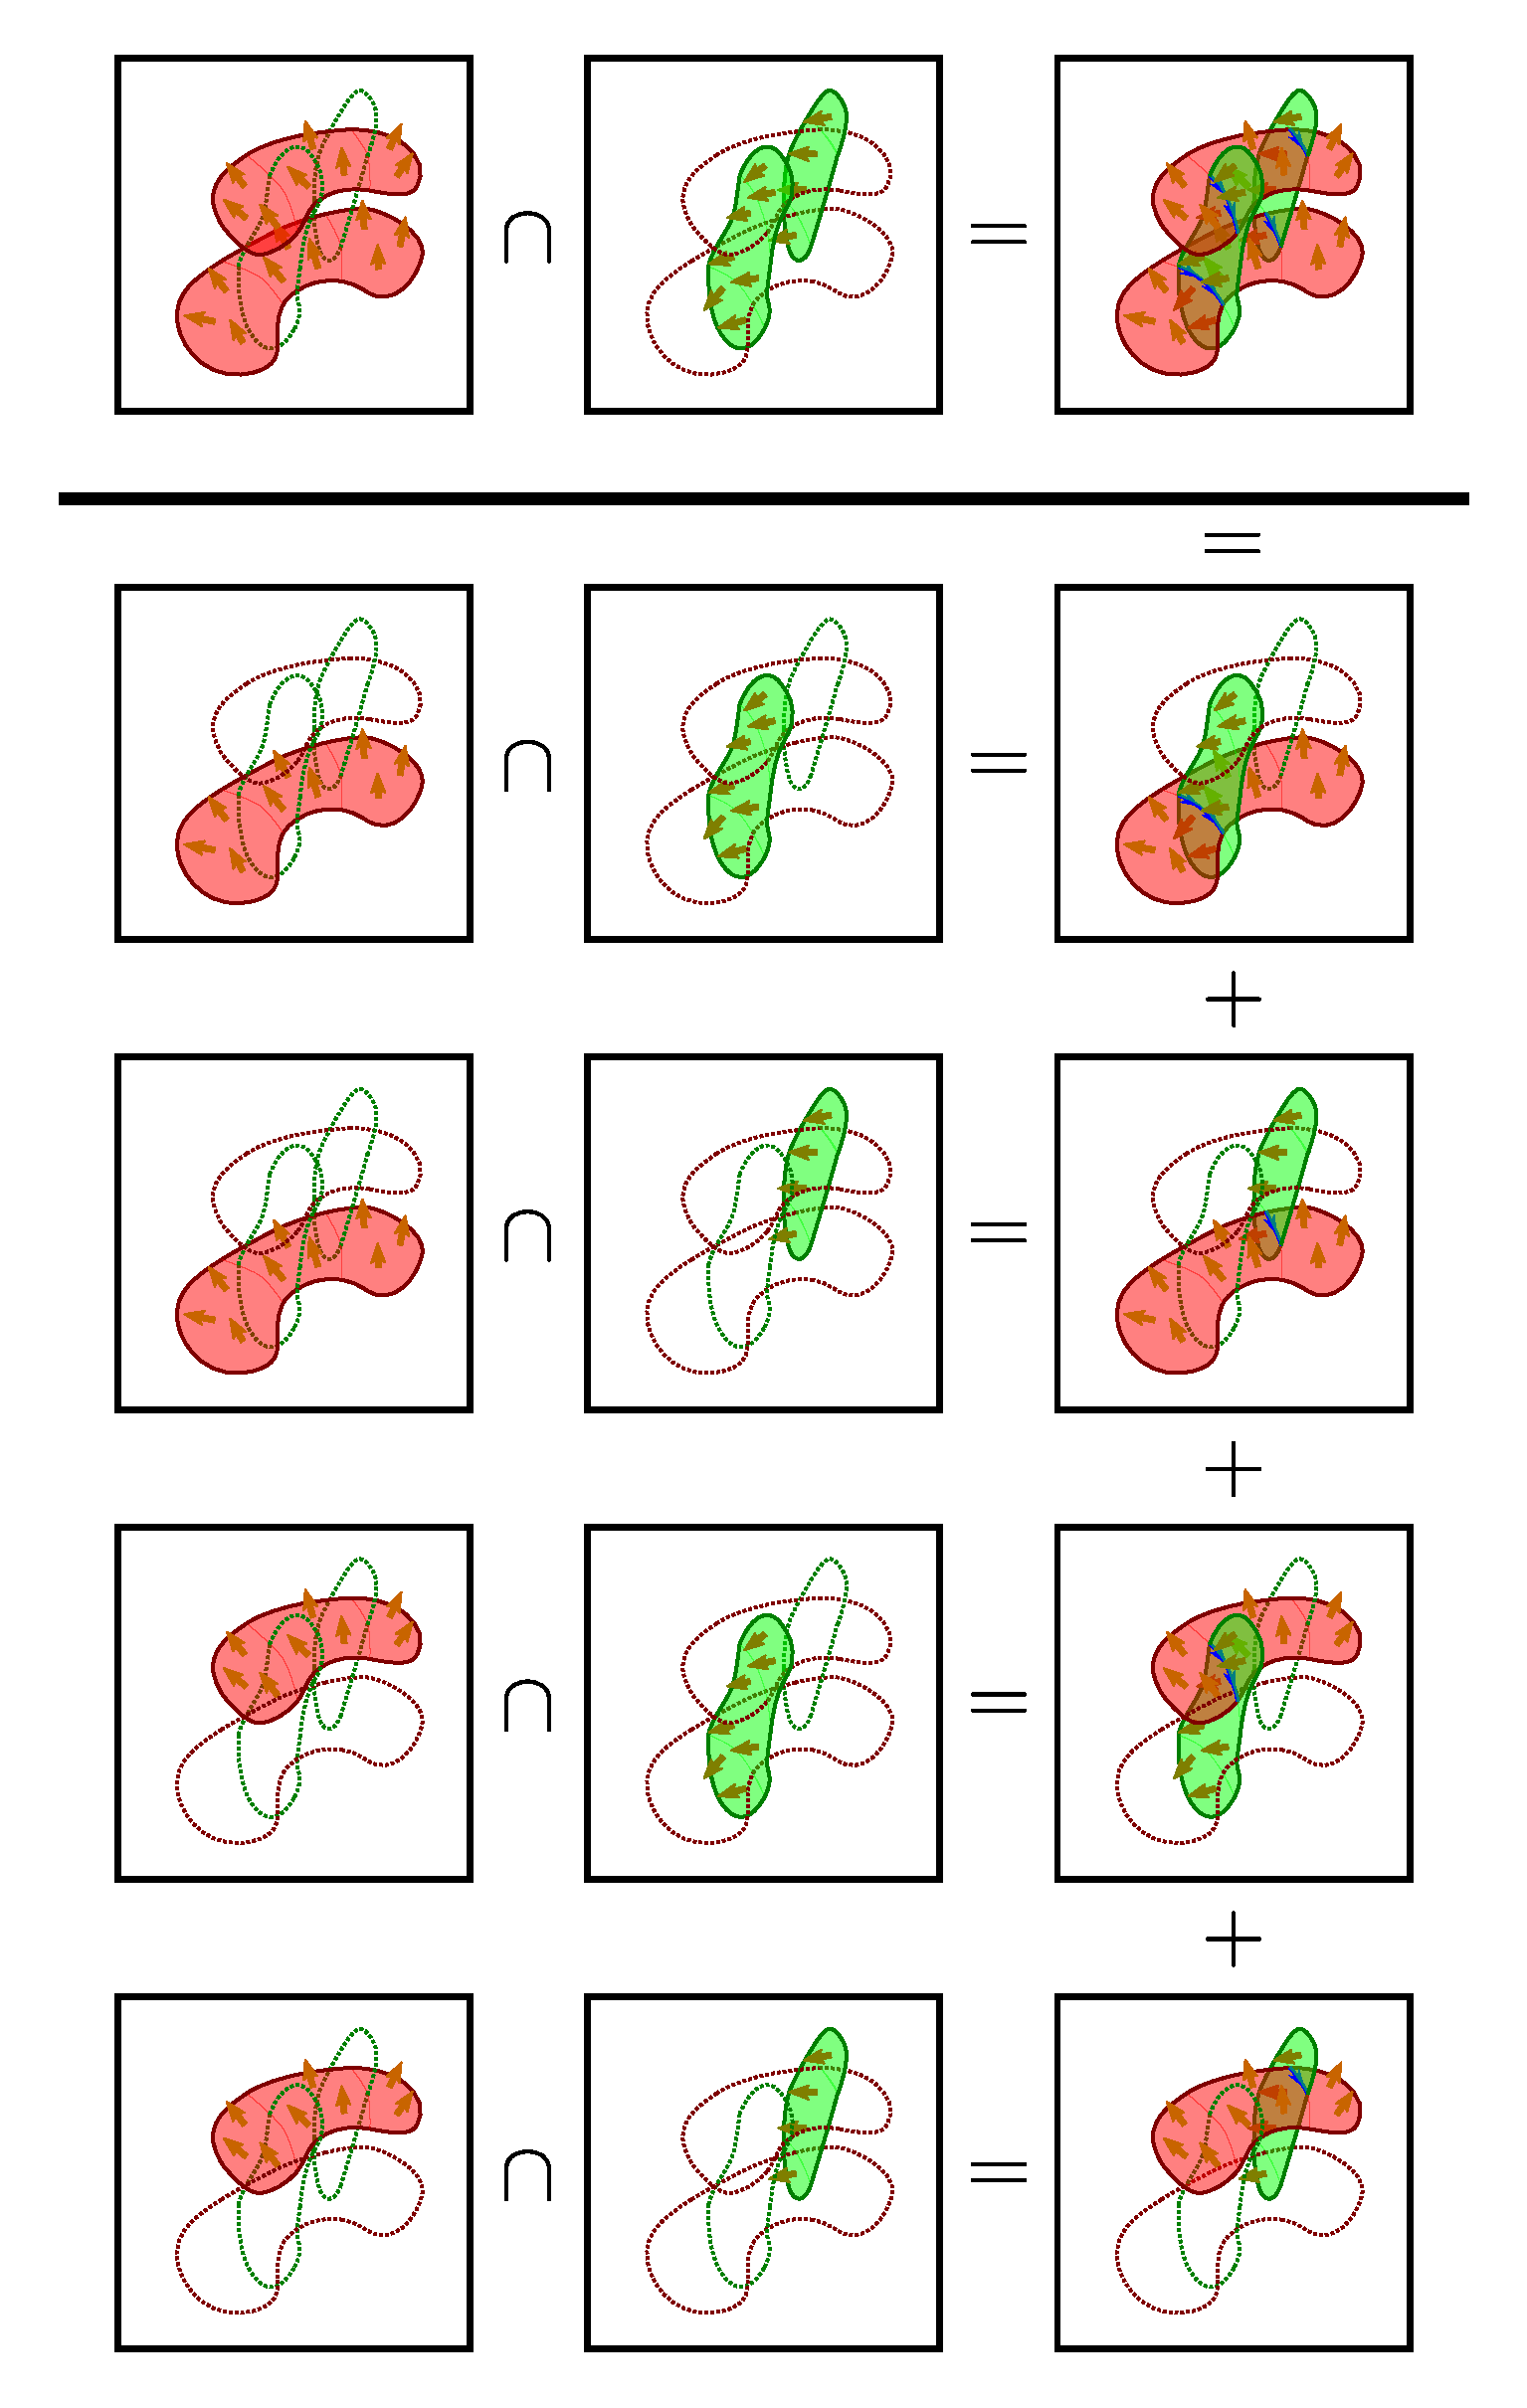
\includegraphics[width = 0.4\textwidth]{Intersections/Surface-surface_intersections/surface_surface_intersection_distributive_law}
}
\end{tabular}
\end{center}

If one surface fails to fully pass through the other surface, then the weight of the intersection path is halved. Surfaces that are embedded inside of other surfaces do contribute any intersection paths unless they enter or leave the other surface. 

Below are examples of surfaces intersecting each other but not fully passing through. Note the bottom example where both surfaces are truncated, so the intersection weight is further halved to \(0.25\).

\begin{center}
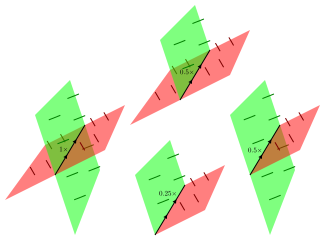
\includegraphics[width = 0.75\textwidth]{Intersections/Surface-surface_intersections/surface_surface_intersection_boundary_case}
\end{center}

Two surfaces that are coincident do not slice through each other and therefore do not intersect. If \(\mathbf{F}_1\) and \(\mathbf{F}_2\) are the same flat surface as depicted below on the left, then these surfaces {\bf do not intersect:} \(\mathbf{F}_1 \times \mathbf{F}_2 = 0\). On the right, the curves where surface \(\mathbf{F}_2\) peels away from \(\mathbf{F}_1\) are intersection curves with weights of \(0.5\).

\begin{center}
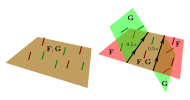
\includegraphics[width = 0.75\textwidth]{Intersections/Surface-surface_intersections/coincident_surfaces}
\end{center}

\begin{tabular}{cc}
\parbox{0.6\textwidth}{
While a surface cannot intersect itself directly as explained above, a surface can still be folded over to explicitly slice through itself as depicted on the right. However, we will soon see that this type of intersection actually does not count, primarily since the intersection cannot be oriented in an objective manner. From a more mathematical perspective, consider the following: Let \(\sigma_1\) and \(\sigma_2\) be two flat surfaces that intersect each other, but with no self intersections that result from folding over. Let multi-surface \(\mathbf{G}\) be comprised of \(\sigma_1\) and \(\sigma_2\):
\[\mathbf{G} = \sigma_1 + \sigma_2\] 
} & \parbox{0.4\textwidth}{
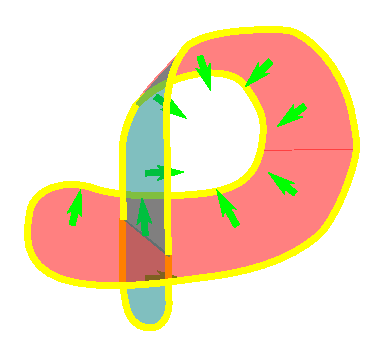
\includegraphics[width = 0.4\textwidth]{Intersections/Surface-surface_intersections/folded_surface_self_intersection}
}
\end{tabular}
The intersection of \(\mathbf{G}\) with itself is: 
\begin{align*}
\mathbf{G} \times \mathbf{G} = (\sigma_1 + \sigma_2) \times (\sigma_1 + \sigma_2) = (\sigma_1 \times \sigma_1) + (\sigma_1 \times \sigma_2) + (\sigma_2 \times \sigma_1) + (\sigma_2 \times \sigma_2)
\end{align*}

We've already established that for surfaces that do not have any self intersections from folding, do not intersect themselves in any other manner, so \(\sigma_1 \times \sigma_1 = 0\) and \(\sigma_2 \times \sigma_2 = 0\). It is also the case that reversing the order of \(\sigma_1\) and \(\sigma_2\) flips the orientation so \(\sigma_2 \times \sigma_1 = -(\sigma_1 \times \sigma_2)\). Therefore: 
\[\mathbf{G} \times \mathbf{G} = 0 + (\sigma_1 \times \sigma_2) + (\sigma_2 \times \sigma_1) + 0 = (\sigma_1 \times \sigma_2) - (\sigma_1 \times \sigma_2) = 0\]

%\begin{center}
%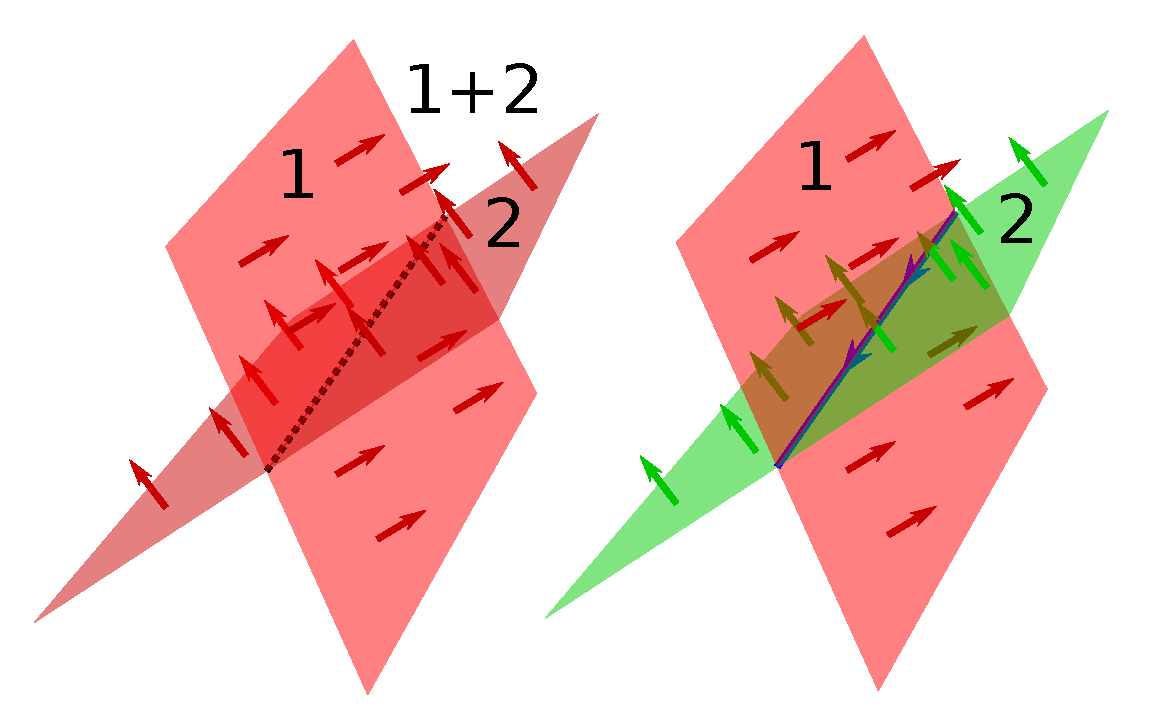
\includegraphics[width = 0.75\textwidth]{Intersections/Surface-surface_intersections/surface_self_intersections}
%\end{center}

In general, the intersection of a multi-surface with itself is always \(0\):

\begin{thm}
\[\mathbf{F} \times \mathbf{F} = 0\]
\end{thm}


Lastly, 3 multi-surface surfaces intersect at a multi-point. Consider \(3\) multi-surfaces \(\mathbf{F}\), \(\mathbf{G}\), and \(\mathbf{H}\). The intersection between \(\mathbf{F}\) and \(\mathbf{G}\) is the multi-path \(\mathbf{F} \times \mathbf{G}\). The intersection between the multi-path \(\mathbf{F} \times \mathbf{G}\) and multi-surface \(\mathbf{H}\) is the multi-point \((\mathbf{F} \times \mathbf{G}) \bullet \mathbf{H}\). This intersection can also be generated by computing the intersection of \(\mathbf{G}\) and \(\mathbf{H}\) first, or the intersection of \(\mathbf{H}\) and \(\mathbf{F}\) first:
\[(\mathbf{F} \times \mathbf{G}) \bullet \mathbf{H} = (\mathbf{G} \times \mathbf{H}) \bullet \mathbf{F} = (\mathbf{H} \times \mathbf{F}) \bullet \mathbf{G}\]
Note that swapping any two surfaces in the above intersections flips the polarity of the intersection point:
\begin{thm}
\begin{align*}
& (\mathbf{F} \times \mathbf{G}) \bullet \mathbf{H} = (\mathbf{G} \times \mathbf{H}) \bullet \mathbf{F} = (\mathbf{H} \times \mathbf{F}) \bullet \mathbf{G} \\ 
= & -(\mathbf{G} \times \mathbf{F}) \bullet \mathbf{H} = -(\mathbf{H} \times \mathbf{G}) \bullet \mathbf{F} = -(\mathbf{F} \times \mathbf{H}) \bullet \mathbf{G}
\end{align*}
\end{thm}

\begin{tabular}{cc}
\parbox{0.5\textwidth}{
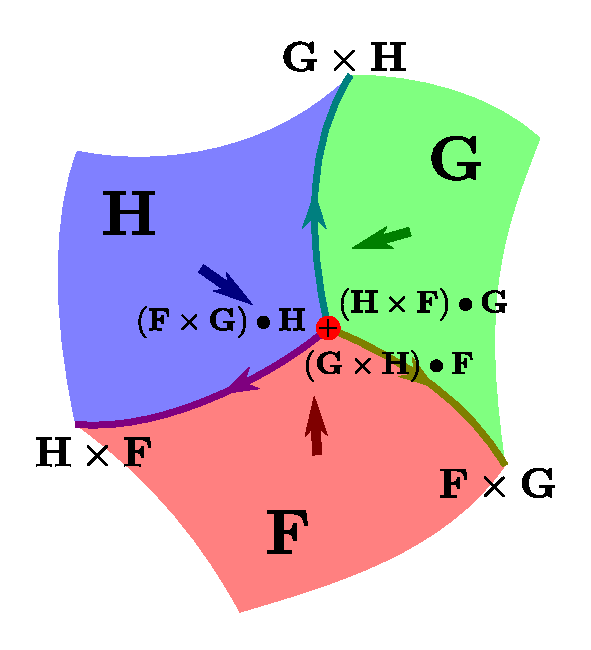
\includegraphics[width = 0.5\textwidth]{Intersections/Surface-surface_intersections/surface_surface_surface_intersections}
} & \parbox{0.5\textwidth}{
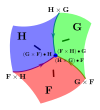
\includegraphics[width = 0.5\textwidth]{Intersections/Surface-surface_intersections/surface_surface_surface_intersections_reversed}
}
\end{tabular}

It was previously noted that a path only ``intersects" a surface when it decisively passes through the surface, and that paths that are embedded within surfaces do not contribute any intersection points. Since the intersection path \(\mathbf{F} \times \mathbf{G}\) is embedded in surfaces \(\mathbf{F}\) and \(\mathbf{G}\), then contrary to intuition, there is no intersection of \(\mathbf{F} \times \mathbf{G}\) with either \(\mathbf{F}\) or \(\mathbf{G}\):
\begin{thm}
\[\mathbf{F} \bullet (\mathbf{F} \times \mathbf{G}) = 0 \quad\quad\quad\text{and}\quad\quad\quad \mathbf{G} \bullet (\mathbf{F} \times \mathbf{G}) = 0\]  
\end{thm}




\section{Surface-volume intersections} 

Given a multi-surface \(\mathbf{F}\) and a multi-volume \(U\), then the intersection between \(\mathbf{F}\) and \(U\) is a multi-surface and is denoted by:

\[\mathbf{F} \cdot U \quad\quad\text{or}\quad\quad \mathbf{F} U \quad\quad\text{or}\quad\quad U \cdot \mathbf{F} \quad\quad\text{or}\quad\quad U \mathbf{F}\]

Given an oriented surface \(\sigma\), and a volume \(\Omega\), then the intersection is the sections of \(\sigma\) that are contained in \(\Omega\). If the weight of \(\Omega\) is negative, then the orientation of the intersection is reversed.  

In the examples below, only sections of the surface that are contained inside a volume are part of the intersection. In the example on the right, because the volume of weight is negative, the orientation is reversed

\begin{center}
\begin{tabular}{cc}
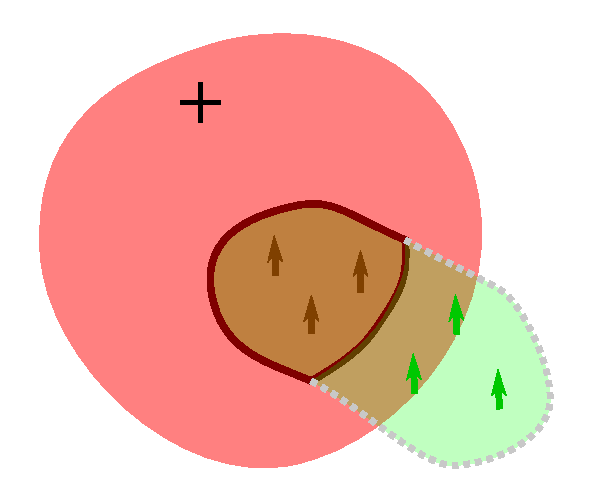
\includegraphics[width = 0.3\textwidth]{Intersections/Surface-volume_intersections/surface_volume_intersections_example_1}
& 
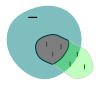
\includegraphics[width = 0.3\textwidth]{Intersections/Surface-volume_intersections/surface_volume_intersections_example_2}
\end{tabular}
\end{center}

If a surface \(\sigma\) with a nonnegative weight of \(w_1\) intersects a volume \(\Omega\) with a weight of \(w_2\) and \(\sigma'\) is the sections of \(\sigma\) that are contained in \(\Omega\), then for each of the \(w_2\) copies of \(\Omega\), \(w_1\) copies of \(\sigma\) are intersecting that copy. The total intersection is \(w_1 \cdot w_2\) copies of \(\sigma'\):
\[(w_1 \sigma) \cdot (w_2 \Omega) = w_1 w_2 \sigma'\] 
If the volume weight \(w_2\) is negative, then both the orientation of \(\sigma'\) and the sign of the weight \(w_1 w_2\) is flipped. 

Given a multi-surface \(\mathbf{F} = w_1\sigma_1 + w_2\sigma_2 + ... + w_N\sigma_N\) and a multi-volume \\ \(U = v_1\Omega_1 + v_2\Omega_2 + ... + v_M\Omega_M\), then the intersection \(\mathbf{F} \cdot U\) is the set of all pairwise intersections of the surfaces and volumes:
\begin{align*}
\mathbf{F} \cdot U = & \left\{\begin{array}{c}
\;\; w_1 v_1 (\sigma_1 \cdot \Omega_1) + w_1 v_2 (\sigma_1 \cdot \Omega_2) + \cdots + w_1 v_M (\sigma_1 \cdot \Omega_M) \\ 
+ w_2 v_1 (\sigma_2 \cdot \Omega_1) + w_2 v_2 (\sigma_2 \cdot \Omega_2) + \cdots + w_2 v_M (\sigma_2 \cdot \Omega_M) \\ 
\vdots \\
+ w_N v_1 (\sigma_N \cdot \Omega_1) + w_N v_2 (\sigma_N \cdot \Omega_2) + \cdots + w_N v_M (\sigma_N \cdot \Omega_M) \\ 
\end{array}\right.
\end{align*}

In general,
\begin{itemize}
\item Given multi-surfaces \(\mathbf{F}_1\) and \(\mathbf{F}_2\), and multi-volume \(U\), then:
\[(\mathbf{F}_1 + \mathbf{F}_2) \cdot U = \mathbf{F}_1 \cdot U + \mathbf{F}_2 \cdot U\] 
\item Given multi-surface \(\mathbf{F}\), multi-volume \(U\), and some real number \(c\), then:
\[(c\mathbf{F}) \cdot U = c(\mathbf{F} \cdot U)\]
\item Given multi-surface \(\mathbf{F}\), and multi-volumes \(U_1\) and \(U_2\), then:
\[\mathbf{F} \cdot (U_1 + U_2) = \mathbf{F} \cdot U_1 + \mathbf{F} \cdot U_2\] 
\item Given multi-surface \(\mathbf{F}\), multi-volume \(U\), and some real number \(c\), then:
\[\mathbf{F} \cdot (cU) = c(\mathbf{F} \cdot U)\]
\end{itemize}

In the example below, the multi-volume \(U\) consists of three volumes. Two of the volumes have a weight of \(+1\) and are overlapping, and the remaining separate volume has a weight of \(-1\). The multi-path \(\mathbf{F}\) consists of a single surface that slices through all of the volumes. Outside of all of the volumes, the surface is not part of the intersection. Where the surface is inside a single volume with a weight of \(+1\), the intersection surface from \(\mathbf{F} \cdot U\) has a weight of \(+1\). Where the surface is inside the overlap between the volumes with a weight of \(+1\), then each volume contributes a copy of the intersection to \(\mathbf{F} \cdot U\) so the weight of the surface in \(\mathbf{F} \cdot U\) is \(+2\). Where the surface is inside the volume with a weight of \(-1\), the orientation of the intersection is reversed.  

\begin{center}
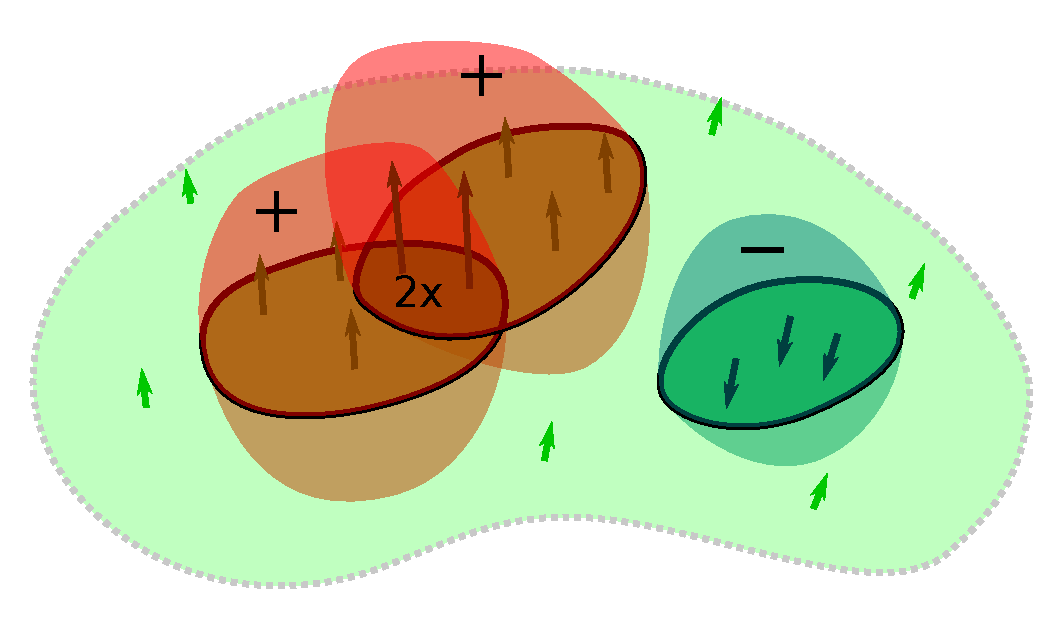
\includegraphics[width = 0.75\textwidth]{Intersections/Surface-volume_intersections/surface_volume_intersections_example_3}
\end{center}

\begin{tabular}{cc}
\parbox{0.5\textwidth}{
If a surface \(\sigma\) is on the surface of volume \(\Omega\), then the intersection is \(\sigma\) with a weight of \(+0.5\) as depicted on the right.
} & \parbox{0.5\textwidth}{
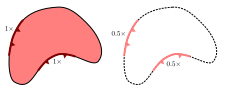
\includegraphics[width = 0.5\textwidth]{Intersections/Surface-volume_intersections/surface_volume_intersection_boundary_case}
}
\end{tabular}





\section{Volume-volume intersections}

Given two multi-volumes \(U_1\) and \(U_2\), then the intersection between \(U_1\) and \(U_2\) is a multi-volume and is denoted by:

\[U_1 \cdot U_1 \quad\quad\text{or}\quad\quad U_1 U_2\]

Given volumes \(\Omega_1\) and \(\Omega_2\), then the intersection is the sections of \(\Omega_1\) and \(\Omega_2\) that overlap. 

If a volume \(\Omega_1\) with a weight of \(w_1\) intersects a volume \(\Omega_2\) with a weight of \(w_2\) and \(\Omega'\) is the sections of \(\Omega_1\) and \(\Omega_2\) that overlap, then for each of the \(w_2\) copies of \(\Omega_2\), \(w_1\) copies of \(\Omega_1\) are intersecting that copy. The total intersection is \(w_1 \cdot w_2\) copies of \(\Omega'\):
\[(w_1\Omega_1) \cdot (w_2\Omega_2) = w_1 w_2 \Omega'\] 

Given multi-volumes \(U_1 = w_1\Omega_1 + w_2\Omega_2 + ... + w_N\Omega_N\) and \\ \(U_2 = v_1\Phi_1 + v_2\Phi_2 + ... + v_M\Phi_M\), then the intersection \(U_1 \cdot U_2\) is the set of all pairwise intersections of the volumes:
\begin{align*}
U_1 \cdot U_2 = & \left\{\begin{array}{c}
\;\; w_1 v_1 (\Omega_1 \cdot \Phi_1) + w_1 v_2 (\Omega_1 \cdot \Phi_2) + \cdots + w_1 v_M (\Omega_1 \cdot \Phi_M) \\ 
+ w_2 v_1 (\Omega_2 \cdot \Phi_1) + w_2 v_2 (\Omega_2 \cdot \Phi_2) + \cdots + w_2 v_M (\Omega_2 \cdot \Phi_M) \\ 
\vdots \\
+ w_N v_1 (\Omega_N \cdot \Phi_1) + w_N v_2 (\Omega_N \cdot \Phi_2) + \cdots + w_N v_M (\Omega_N \cdot \Phi_M) \\ 
\end{array}\right.
\end{align*}

In general,
\begin{itemize}
\item Given multi-volumes \(U_1\), \(U_2\), and \(V\), then:
\[(U_1 + U_2) \cdot V = U_1 \cdot V + U_2 \cdot V\] 
\item Given multi-volumes \(U\) and \(V\), and some real number \(c\), then:
\[(cU) \cdot V = c(U \cdot V)\]
\item Given multi-volumes \(U\), \(V_1\), and \(V_2\), then:
\[U \cdot (V_1 + V_2) = U \cdot V_1 + U \cdot V_2\] 
\item Given multi-volumes \(U\) and \(V\), and some real number \(c\), then:
\[U \cdot (cV) = c(U \cdot V)\]
\end{itemize}

Some examples of intersecting multi-volumes are shown below. Note that for a specific point \(\mathbf{q}\), that the net number of volumes that contain \(\mathbf{q}\) in the intersection \(U_1 \cdot U_2\) will always be the product of the net number of volumes that contain \(\mathbf{q}\) in each of \(U_1\) and \(U_2\):
\[(U_1 \cdot U_2)(\mathbf{q}) = U_1(\mathbf{q}) \cdot U_2(\mathbf{q})\]

\begin{center}
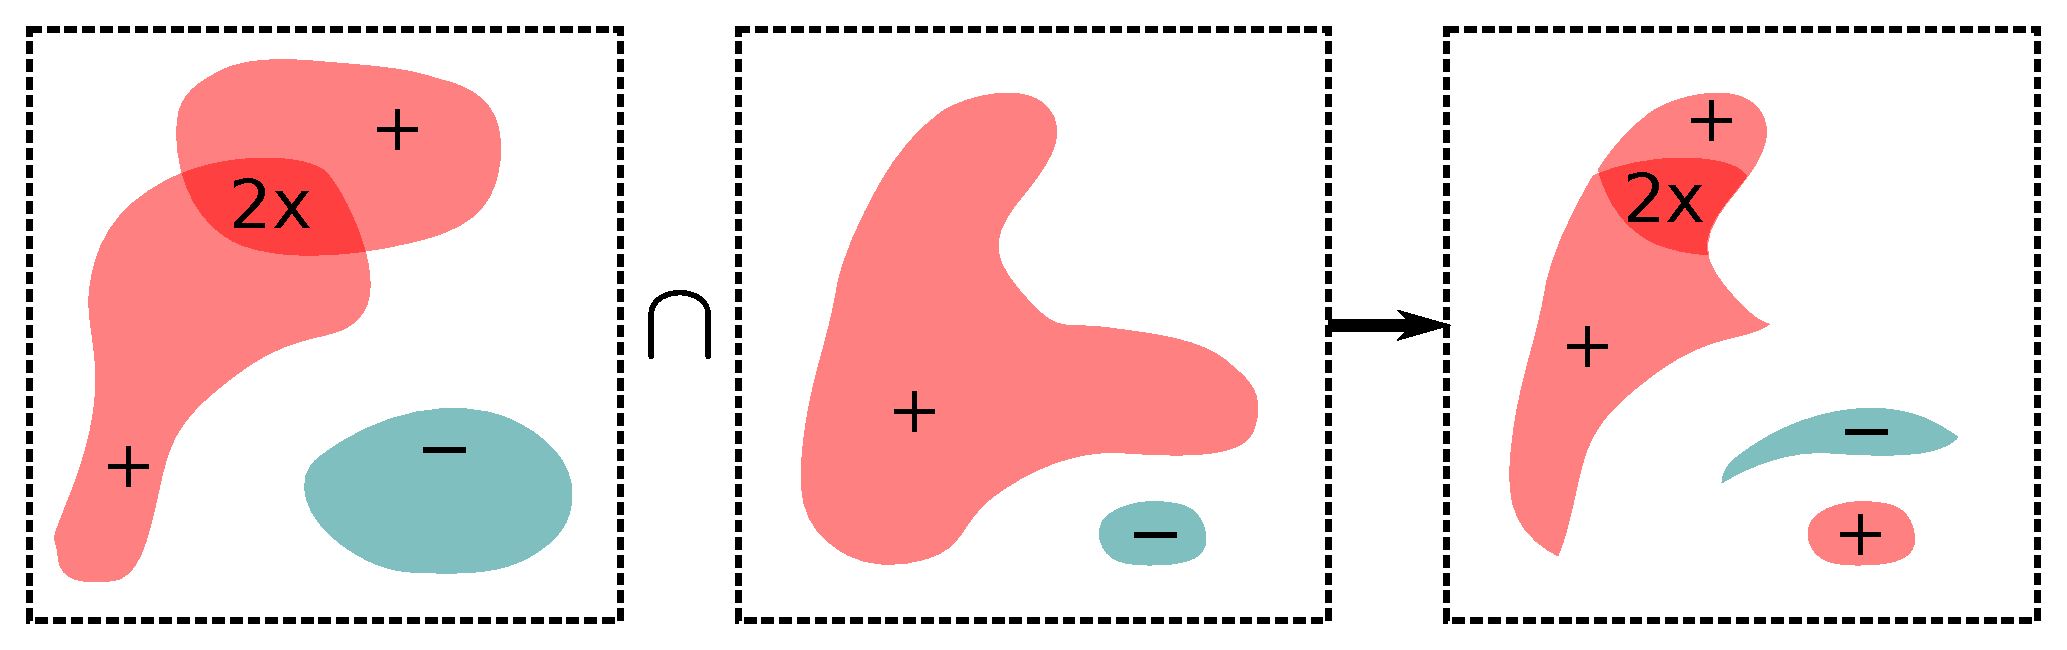
\includegraphics[width = \textwidth]{Intersections/Volume-volume_intersections/volume_volume_intersections_three_panel_example}
\end{center}

\begin{center}
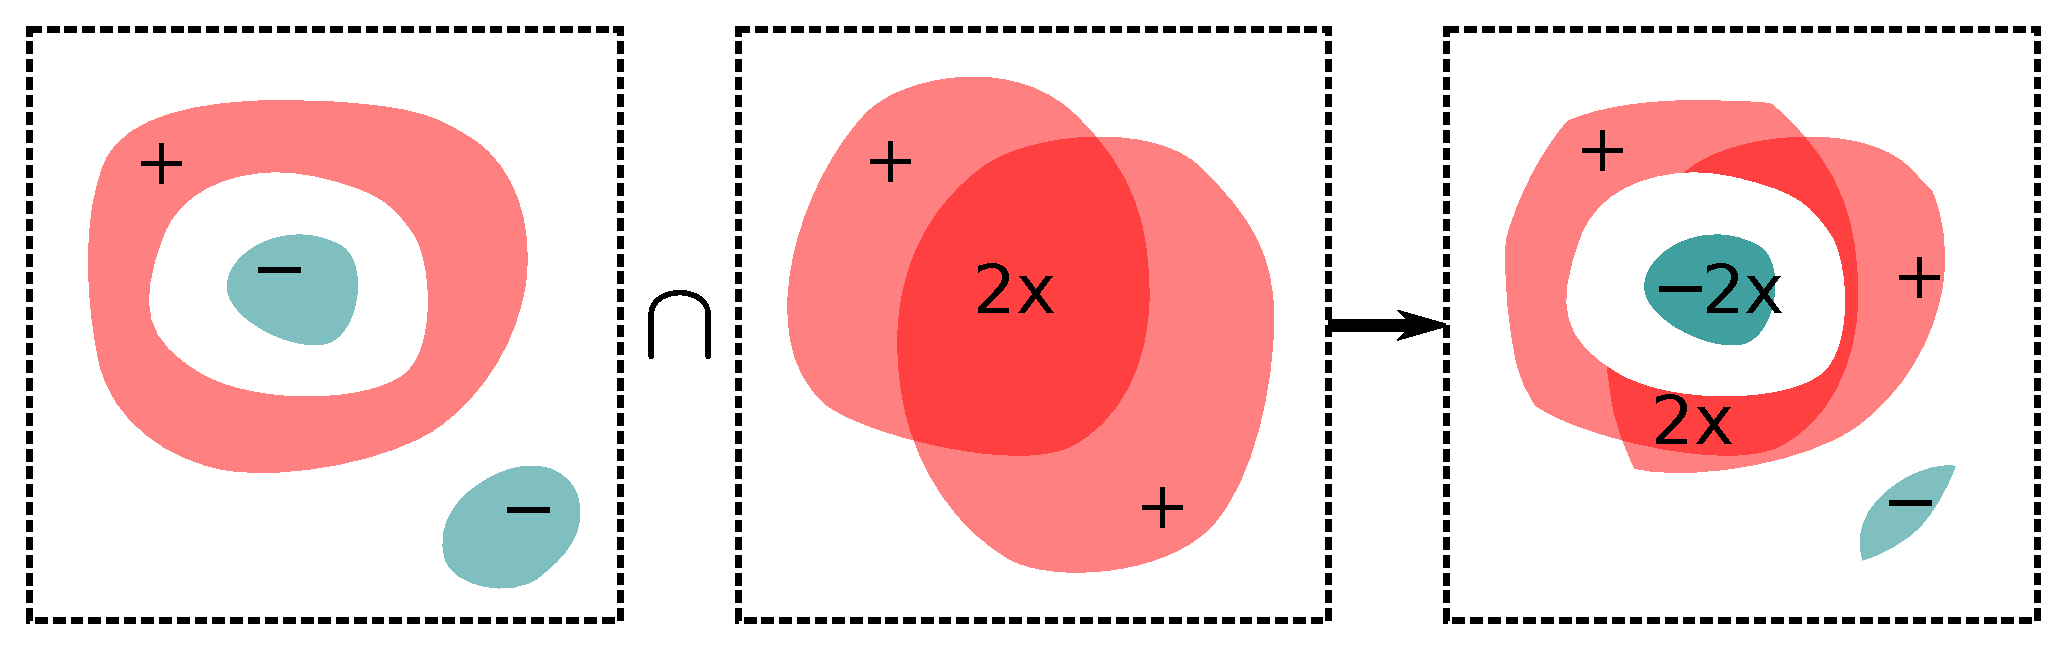
\includegraphics[width = \textwidth]{Intersections/Volume-volume_intersections/volume_volume_intersections_three_panel_example_2}
\end{center}




\section{Intersections that are not being considered}

What about the following other types of intersections? Namely point-point intersections, point-path intersections, point-surface intersections, and path-path intersections? With the exception of point-point intersections, these intersections cannot be oriented as will be discussed: 


\subsection{Point-path intersections}

%\begin{tabular}{cc}
%\parbox{0.5\textwidth}{
%Consider a point \(P\) and an oriented path \(C\) that passes through point \(P\). The intersection of \(P\) with \(C\) consists of just \(P\), but what weight should point \(P\) have in the intersection?
%\[P \cap C = ?P\]
%It may seem obvious that this weight should simply be \(1\), but consider the path \(-C\), which is path \(C\) with the orientation reversed. \(-C\) also passes through point \(P\) so the intersection point \(P\) should also have a weight of \(1\). In fact, the weight of \(P\) in the intersection \(P \cap C\) should be equal to the weight of \(P\) in the intersection \(P \cap (-C)\).
%\begin{align*}
%& P \cap C  
%= ?P 
%= P \cap (-C)
%\end{align*} 
%} & \parbox{0.5\textwidth}{
%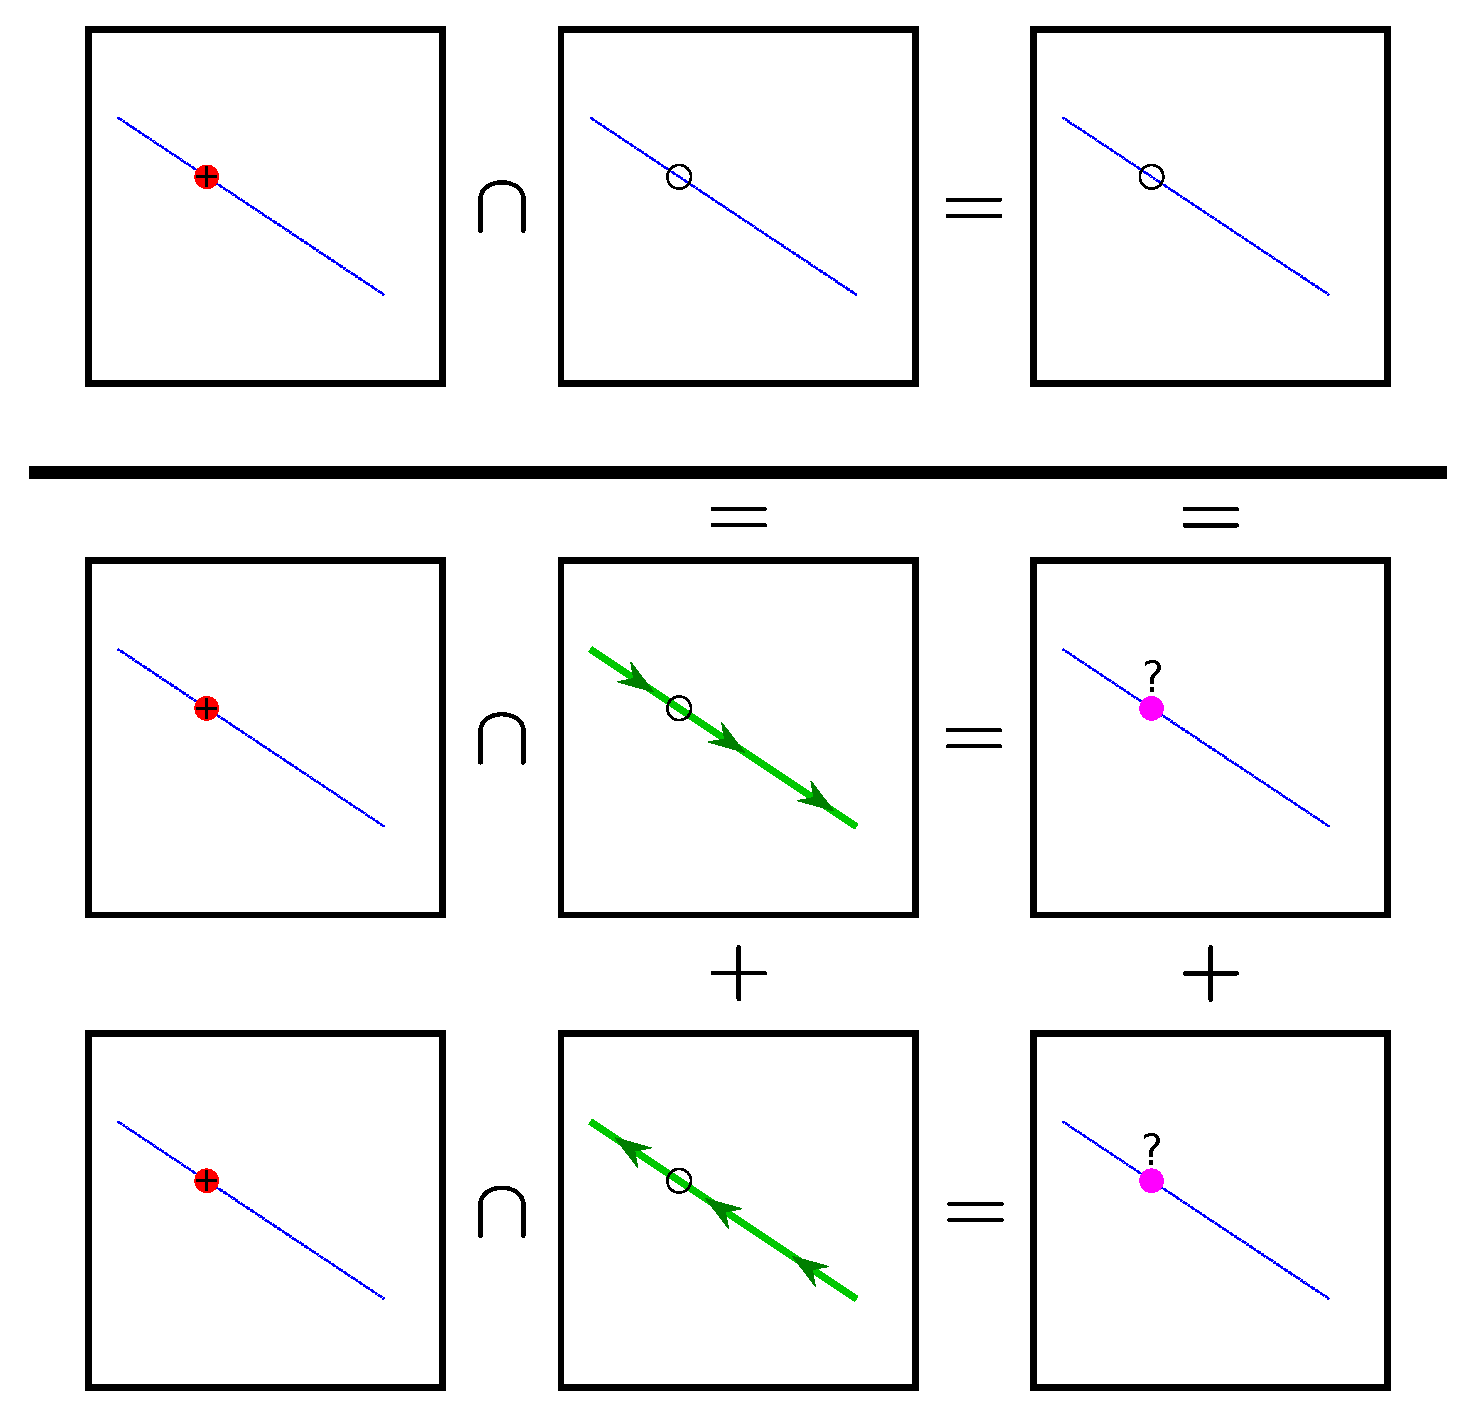
\includegraphics[width = 0.5\textwidth]{Intersections/Undefined_intersections/point_path_intersection_contradiction}
%}
%\end{tabular}
%
%\vspace{5mm}
%
%By linearity, the intersection of \(P\) with the union of \(C\) and \(-C\) is the union of the intersection of \(P\) with \(C\) and the intersection of \(P\) with \(-C\):
%\begin{align*}
%& P \cap \Big(C + (-C)\Big) = P \cap C + P \cap (-C)
%\end{align*}
%Since \(P \cap C = P \cap (-C) = ?P\), 
%\begin{align*}
%P \cap C + P \cap (-C) = ?P + ?P = (2?)P
%\end{align*}
%so the intersection of \(P\) with the union of \(C\) and \(-C\) is 
%\[P \cap \Big(C + (-C)\Big) = (2?)P\]
%
%The union of \(C\) and \(-C\) should be nothing: 
%\[C + (-C) = 0\]  
%
%The intersection of \(P\) with nothing is nothing, so
%\[P \cap \Big(C + (-C)\Big) = P \cap 0 = 0\]  
%
%Therefore, 
%\begin{align*}
%& P \cap \Big(C + (-C)\Big) = (2?)P \quad\quad\text{and}\quad\quad P \cap \Big(C + (-C)\Big) = 0 \quad\quad\text{so}\quad\quad (2?)P = 0 \\ 
%& \quad\quad\text{so}\quad\quad ? = 0
%\end{align*}
%so the weight of point \(P\) in the intersections \(P \cap C\) and \(P \cap (-C)\) can only be \(0\). There cannot be any intersection of a point with a path, in a similar manner to how an oriented surface cannot intersect itself as discussed previously.

Why can't point-path intersections be oriented? Let \(P\) be a point and let \(C\) be an oriented path, where point \(P\) lies on \(C\). Let the weights of \(P\) and \(C\) both be \(1\). What weight should point \(P\) have in the intersection? Should the orientation of \(C\) be reversed, the sign of the weight should also be flipped. Now slowly rotate \(C\) around while maintaining the intersection as depicted below. No matter the direction in which \(C\) passes through \(P\) the weight should ideally remain constant as all directions are equal. The question is at what point during the rotation does the sign of the weight flip? The answer is that the weight should always be \(0\), and the intersection does not exist.  

\begin{center}
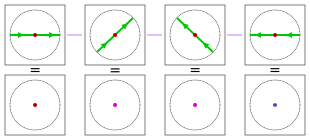
\includegraphics[width = \textwidth]{Intersections/Undefined_intersections/point_path_intersection_contradiction_2}
\end{center}




\subsection{Point-surface intersections}

%\begin{tabular}{cc}
%\parbox{0.5\textwidth}{
%Consider a point \(P\) and an oriented surface \(\sigma\) that passes through point \(P\). The intersection of \(P\) with \(\sigma\) consists of just \(P\), but what weight should point \(P\) have in the intersection?
%\[P \cap \sigma = ?P\]
%It may seem obvious that this weight should simply be \(1\), but consider the surface \(-\sigma\), which is surface \(\sigma\) with the orientation reversed. \(-\sigma\) also passes through point \(P\) so the intersection point \(P\) should also have a weight of \(1\). In fact, the weight of \(P\) in the intersection \(P \cap \sigma\) should be equal to the weight of \(P\) in the intersection \(P \cap (-\sigma)\).
%\begin{align*}
%& P \cap \sigma  
%= ?P 
%= P \cap (-\sigma)  
%\end{align*} 
%} & \parbox{0.5\textwidth}{
%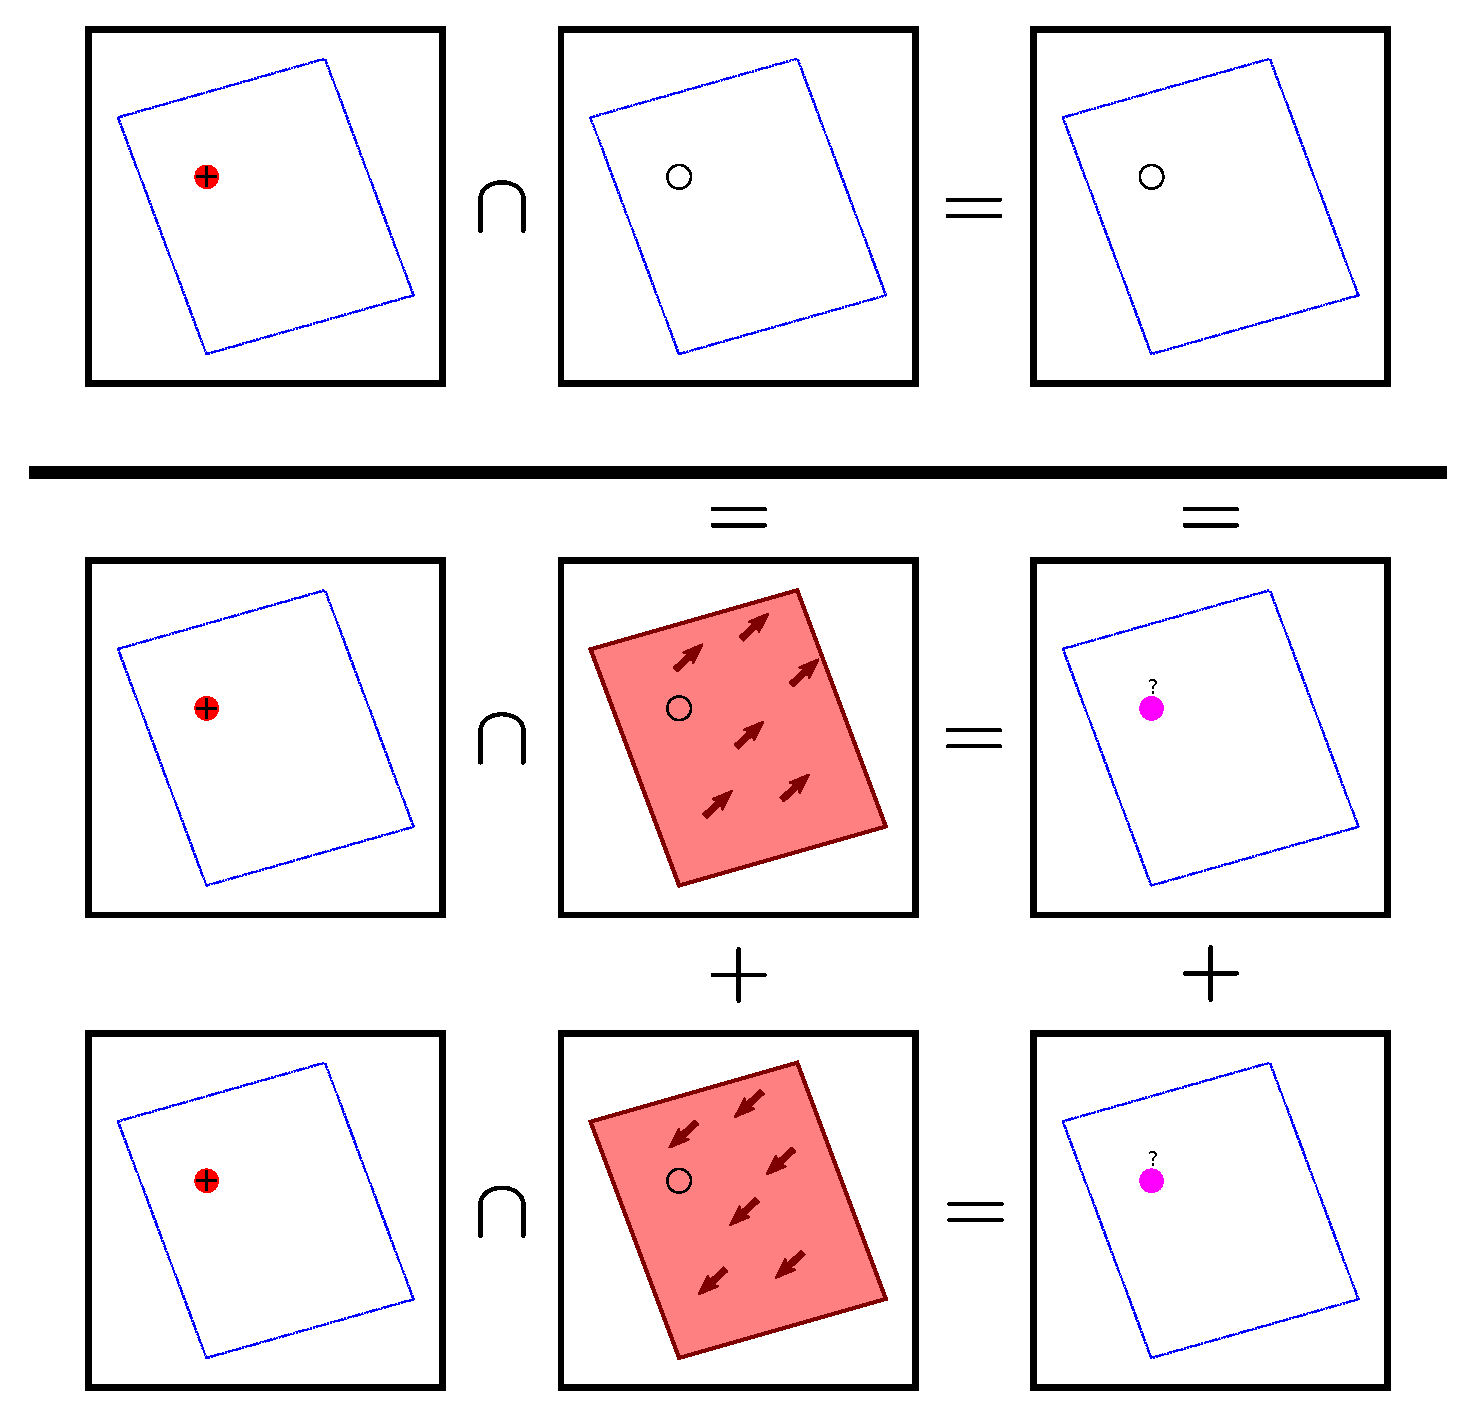
\includegraphics[width = 0.5\textwidth]{Intersections/Undefined_intersections/point_surface_intersection_contradiction}
%}
%\end{tabular}
%
%\vspace{5mm}
%
%By linearity, the intersection of \(P\) with the union of \(\sigma\) and \(-\sigma\) is the union of the intersection of \(P\) with \(\sigma\) and the intersection of \(P\) with \(-\sigma\):
%\begin{align*}
%& P \cap \Big(\sigma + (-\sigma)\Big) = P \cap \sigma + P \cap (-\sigma)
%\end{align*}
%Since \(P \cap \sigma = P \cap (-\sigma) = ?P\), 
%\begin{align*}
%P \cap \sigma + P \cap (-\sigma) = ?P + ?P = (2?)P  
%\end{align*}
%so the intersection of \(P\) with the union of \(\sigma\) and \(-\sigma\) is 
%\[P \cap \Big(\sigma + (-\sigma)\Big) = (2?)P\]
%
%The union of \(\sigma\) and \(-\sigma\) should be nothing: 
%\[\sigma + (-\sigma) = 0\]
%
%The intersection of \(P\) with nothing is nothing, so
%\[P \cap \Big(\sigma + (-\sigma)\Big) = P \cap 0 = 0\]  
%
%Therefore, 
%\begin{align*}
%& P \cap \Big(\sigma + (-\sigma)\Big) = (2?)P \quad\quad\text{and}\quad\quad P \cap \Big(\sigma + (-\sigma)\Big) = 0 \quad\quad\text{so}\quad\quad (2?)P = 0 \\ 
%& \quad\quad\text{so}\quad\quad ? = 0
%\end{align*}
%so the weight of point \(P\) in the intersections \(P \cap \sigma\) and \(P \cap (-\sigma)\) can only be \(0\). There cannot be any intersection of a point with a surface, in a similar manner to how an oriented surface cannot intersect itself as discussed previously.

Why can't point-surface intersections be oriented? Let \(P\) be a point and let \(\sigma\) be an oriented surface, where point \(P\) lies on \(\sigma\). Let the weights of \(P\) and \(\sigma\) both be \(1\). What weight should point \(P\) have in the intersection? Should the orientation of \(\sigma\) be reversed, the sign of the weight should also be flipped. Now slowly rotate \(\sigma\) around while maintaining the intersection as depicted below. No matter the direction in which \(\sigma\) faces as it passes through \(P\) the weight should ideally remain constant as all directions are equal. The question is at what point during the rotation does the sign of the weight flip? The answer is that the weight should always be \(0\), and the intersection does not exist.  

\begin{center}
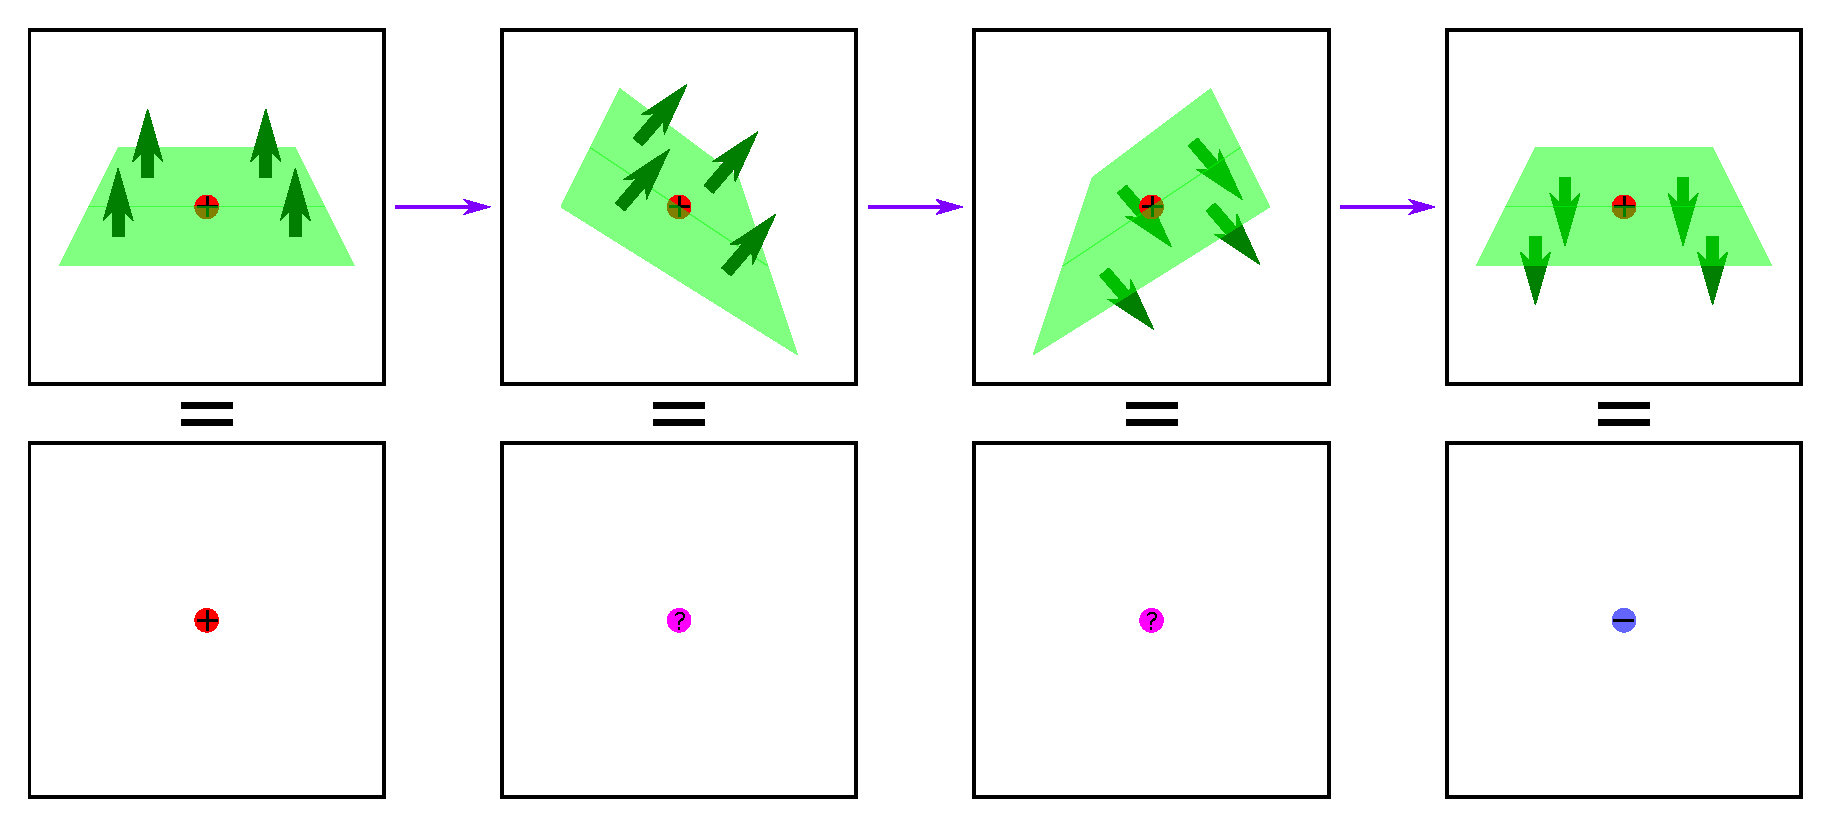
\includegraphics[width = \textwidth]{Intersections/Undefined_intersections/point_surface_intersection_contradiction_2}
\end{center}



\subsection{Path-path intersections}

%\begin{tabular}{cc}
%\parbox{0.5\textwidth}{
%Consider two paths \(C_1\) and \(C_2\) that intersect at point \(P\). What weight should point \(P\) have in the intersection?
%\[C_1 \cap C_2 = ?P\]
%It may seem obvious that this weight should simply be \(1\), but consider the path \(-C_2\), which is path \(C_2\) with the orientation reversed. \(-C_2\) also intersects \(C_1\) at point \(P\) so the intersection point \(P\) should also have a weight of \(1\). In fact, the weight of \(P\) in the intersection \(C_1 \cap C_2\) should be equal to the weight of \(P\) in the intersection \(C_1 \cap -C_2\).
%\begin{align*}
%& C_1 \cap C_2  
%= ?P 
%= C_1 \cap (-C_2)
%\end{align*} 
%} & \parbox{0.5\textwidth}{
%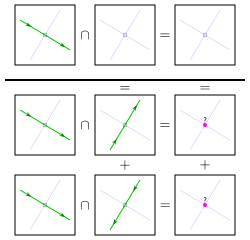
\includegraphics[width = 0.5\textwidth]{Intersections/Undefined_intersections/path_path_intersection_contradiction}
%}
%\end{tabular}
%
%\vspace{5mm}
%
%By linearity, the intersection of \(C_1\) with the union of \(C_2\) and \(-C_2\) is the union of the intersection of \(C_1\) with \(C_2\) and the intersection of \(C_1\) with \(-C_2\):
%\begin{align*}
%& C_1 \cap \Big(C_2 + (-C_2)\Big) = C_1 \cap C_2 + C_1 \cap (-C_2)
%\end{align*}
%Since \(C_1 \cap C_2 = C_1 \cap (-C_2) = ?P\), 
%\begin{align*}
% C_1 \cap C_2 + C_1 \cap (-C_2) = ?P + ?P = (2?)P 
%\end{align*}
%so the intersection of \(C_1\) with the union of \(C_2\) and \(-C_2\) is 
%\[C_1 \cap \Big(C_2 + (-C_2)\Big) = (2?)P\]
%
%The union of \(C_2\) and \(-C_2\) should be nothing: 
%\[C_2 + (-C_2) = 0\]
%
%The intersection of \(C_1\) with nothing is nothing, so
%\[C_1 \cap \Big(C_2 + (-C_2)\Big) = C_1 \cap 0 = 0\]  
%
%Therefore, 
%\begin{align*}
%& C_1 \cap \Big(C_2 + (-C_2)\Big) = (2?)P \quad\quad\text{and}\quad\quad C_1 \cap \Big(C_2 + (-C_2)\Big) = 0 \quad\quad\text{so}\quad\quad (2?)P = 0 \\ 
%& \quad\quad\text{so}\quad\quad ? = 0
%\end{align*}
%so the weight of point \(P\) in the intersections \(C_1 \cap C_2\) and \(C_1 \cap (-C_2)\) can only be \(0\). There cannot be any intersection of a path with a path, in a similar manner to how an oriented surface cannot intersect itself as discussed previously.

Why can't path-path intersections be oriented? Let \(C_1\) and \(C_2\) be oriented paths that intersect at point \(P\). Let the weights of \(C_1\) and \(C_2\) both be \(1\). What weight should point \(P\) have in the intersection? Should the orientation of \(C_1\) xor \(C_2\) be reversed, the sign of the weight should also be flipped. Now slowly rotate \(C_2\) around while maintaining the intersection as depicted below. Also, at no point during the rotation \(C_2\) will have the same direction of \(C_1\). No matter the direction in which \(C_2\) intersects \(C_1\) the weight should ideally remain constant as all directions are equal (except if \(C_1\) and \(C_2\) share the same direction). The question is at what point during the rotation does the sign of the weight flip? The answer is that the weight should always be \(0\), and the intersection does not exist.  

\begin{center}
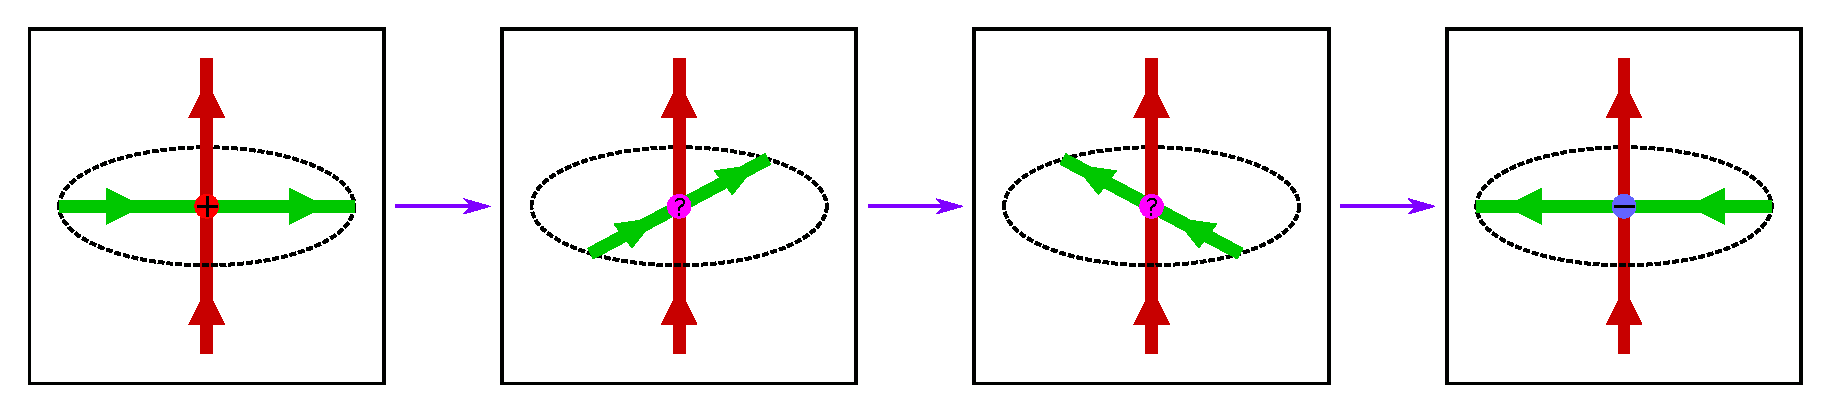
\includegraphics[width = \textwidth]{Intersections/Undefined_intersections/path_path_intersection_contradiction_2}
\end{center}



\section{Summary}

A summary of the notations used for various intersections is given below:

\vspace{5mm}

\begin{tabular}{|c||c|c|c|c|}
\hline
Intersections & point \(\rho_2\) \red{\{0\}} & path \(\mathbf{J}_2\) \red{\{1\}} & surface \(\mathbf{F}_2\) \red{\{2\}} & volume \(U_2\) \red{\{3\}} \\
\hline
\hline
point \(\rho_1\) \red{\{0\}} & 
N/A & 
N/A & 
N/A & 
point \(\rho_1 \cdot U_2\) \red{\{0\}} \\ 
\hline
path \(\mathbf{J}_1\) \red{\{1\}} & 
N/A & 
N/A & 
point \(\mathbf{J}_1 \bullet \mathbf{F}_2\) \red{\{0\}} & 
path \(\mathbf{J}_1 \cdot U_2\) \red{\{1\}} \\ 
\hline
surface \(\mathbf{F}_1\) \red{\{2\}} & 
N/A & 
point \(\mathbf{F}_1 \bullet \mathbf{J}_2\) \red{\{0\}} & 
path \(\mathbf{F}_1 \times \mathbf{F}_2\) \red{\{1\}} & 
surface \(\mathbf{F}_1 \cdot U_2\) \red{\{2\}} \\ 
\hline
volume \(U_1\) \red{\{3\}} & 
point \(U_1 \cdot \rho_2\) \red{\{0\}} & 
path \(U_1 \cdot \mathbf{J}_2\) \red{\{1\}} & 
surface \(U_1 \cdot \mathbf{F}_2\) \red{\{2\}} & 
volume \(U_1 \cdot U_2\) \red{\{3\}} \\
\hline
\end{tabular}

\vspace{5mm}

In \red{red} is indicated the ``dimensionality" of the multi-structure. Points have \(0\) dimensions; paths have \(1\) dimension; surfaces have \(2\) dimensions; and volumes have \(3\) dimensions. The number of dimensions of the intersection is the sum of the dimensions minus \(3\). When the resultant number of dimensions is less than \(0\), the intersection does not exist.




